% Options for packages loaded elsewhere
\PassOptionsToPackage{unicode}{hyperref}
\PassOptionsToPackage{hyphens}{url}
%
\documentclass[
  letterpaper,
  DIV=11,
  numbers=noendperiod]{scrartcl}

\usepackage{amsmath,amssymb}
\usepackage{setspace}
\usepackage{iftex}
\ifPDFTeX
  \usepackage[T1]{fontenc}
  \usepackage[utf8]{inputenc}
  \usepackage{textcomp} % provide euro and other symbols
\else % if luatex or xetex
  \usepackage{unicode-math}
  \defaultfontfeatures{Scale=MatchLowercase}
  \defaultfontfeatures[\rmfamily]{Ligatures=TeX,Scale=1}
\fi
\usepackage{lmodern}
\ifPDFTeX\else  
    % xetex/luatex font selection
\fi
% Use upquote if available, for straight quotes in verbatim environments
\IfFileExists{upquote.sty}{\usepackage{upquote}}{}
\IfFileExists{microtype.sty}{% use microtype if available
  \usepackage[]{microtype}
  \UseMicrotypeSet[protrusion]{basicmath} % disable protrusion for tt fonts
}{}
\makeatletter
\@ifundefined{KOMAClassName}{% if non-KOMA class
  \IfFileExists{parskip.sty}{%
    \usepackage{parskip}
  }{% else
    \setlength{\parindent}{0pt}
    \setlength{\parskip}{6pt plus 2pt minus 1pt}}
}{% if KOMA class
  \KOMAoptions{parskip=half}}
\makeatother
\usepackage{xcolor}
\setlength{\emergencystretch}{3em} % prevent overfull lines
\setcounter{secnumdepth}{5}
% Make \paragraph and \subparagraph free-standing
\makeatletter
\ifx\paragraph\undefined\else
  \let\oldparagraph\paragraph
  \renewcommand{\paragraph}{
    \@ifstar
      \xxxParagraphStar
      \xxxParagraphNoStar
  }
  \newcommand{\xxxParagraphStar}[1]{\oldparagraph*{#1}\mbox{}}
  \newcommand{\xxxParagraphNoStar}[1]{\oldparagraph{#1}\mbox{}}
\fi
\ifx\subparagraph\undefined\else
  \let\oldsubparagraph\subparagraph
  \renewcommand{\subparagraph}{
    \@ifstar
      \xxxSubParagraphStar
      \xxxSubParagraphNoStar
  }
  \newcommand{\xxxSubParagraphStar}[1]{\oldsubparagraph*{#1}\mbox{}}
  \newcommand{\xxxSubParagraphNoStar}[1]{\oldsubparagraph{#1}\mbox{}}
\fi
\makeatother


\providecommand{\tightlist}{%
  \setlength{\itemsep}{0pt}\setlength{\parskip}{0pt}}\usepackage{longtable,booktabs,array}
\usepackage{calc} % for calculating minipage widths
% Correct order of tables after \paragraph or \subparagraph
\usepackage{etoolbox}
\makeatletter
\patchcmd\longtable{\par}{\if@noskipsec\mbox{}\fi\par}{}{}
\makeatother
% Allow footnotes in longtable head/foot
\IfFileExists{footnotehyper.sty}{\usepackage{footnotehyper}}{\usepackage{footnote}}
\makesavenoteenv{longtable}
\usepackage{graphicx}
\makeatletter
\newsavebox\pandoc@box
\newcommand*\pandocbounded[1]{% scales image to fit in text height/width
  \sbox\pandoc@box{#1}%
  \Gscale@div\@tempa{\textheight}{\dimexpr\ht\pandoc@box+\dp\pandoc@box\relax}%
  \Gscale@div\@tempb{\linewidth}{\wd\pandoc@box}%
  \ifdim\@tempb\p@<\@tempa\p@\let\@tempa\@tempb\fi% select the smaller of both
  \ifdim\@tempa\p@<\p@\scalebox{\@tempa}{\usebox\pandoc@box}%
  \else\usebox{\pandoc@box}%
  \fi%
}
% Set default figure placement to htbp
\def\fps@figure{htbp}
\makeatother
% definitions for citeproc citations
\NewDocumentCommand\citeproctext{}{}
\NewDocumentCommand\citeproc{mm}{%
  \begingroup\def\citeproctext{#2}\cite{#1}\endgroup}
\makeatletter
 % allow citations to break across lines
 \let\@cite@ofmt\@firstofone
 % avoid brackets around text for \cite:
 \def\@biblabel#1{}
 \def\@cite#1#2{{#1\if@tempswa , #2\fi}}
\makeatother
\newlength{\cslhangindent}
\setlength{\cslhangindent}{1.5em}
\newlength{\csllabelwidth}
\setlength{\csllabelwidth}{3em}
\newenvironment{CSLReferences}[2] % #1 hanging-indent, #2 entry-spacing
 {\begin{list}{}{%
  \setlength{\itemindent}{0pt}
  \setlength{\leftmargin}{0pt}
  \setlength{\parsep}{0pt}
  % turn on hanging indent if param 1 is 1
  \ifodd #1
   \setlength{\leftmargin}{\cslhangindent}
   \setlength{\itemindent}{-1\cslhangindent}
  \fi
  % set entry spacing
  \setlength{\itemsep}{#2\baselineskip}}}
 {\end{list}}
\usepackage{calc}
\newcommand{\CSLBlock}[1]{\hfill\break\parbox[t]{\linewidth}{\strut\ignorespaces#1\strut}}
\newcommand{\CSLLeftMargin}[1]{\parbox[t]{\csllabelwidth}{\strut#1\strut}}
\newcommand{\CSLRightInline}[1]{\parbox[t]{\linewidth - \csllabelwidth}{\strut#1\strut}}
\newcommand{\CSLIndent}[1]{\hspace{\cslhangindent}#1}

\usepackage{booktabs}
\usepackage{caption}
\usepackage{longtable}
\usepackage{colortbl}
\usepackage{array}
\usepackage{anyfontsize}
\usepackage{multirow}
\KOMAoption{captions}{tableheading}
\makeatletter
\@ifpackageloaded{caption}{}{\usepackage{caption}}
\AtBeginDocument{%
\ifdefined\contentsname
  \renewcommand*\contentsname{Table of contents}
\else
  \newcommand\contentsname{Table of contents}
\fi
\ifdefined\listfigurename
  \renewcommand*\listfigurename{List of Figures}
\else
  \newcommand\listfigurename{List of Figures}
\fi
\ifdefined\listtablename
  \renewcommand*\listtablename{List of Tables}
\else
  \newcommand\listtablename{List of Tables}
\fi
\ifdefined\figurename
  \renewcommand*\figurename{Figure}
\else
  \newcommand\figurename{Figure}
\fi
\ifdefined\tablename
  \renewcommand*\tablename{Table}
\else
  \newcommand\tablename{Table}
\fi
}
\@ifpackageloaded{float}{}{\usepackage{float}}
\floatstyle{ruled}
\@ifundefined{c@chapter}{\newfloat{codelisting}{h}{lop}}{\newfloat{codelisting}{h}{lop}[chapter]}
\floatname{codelisting}{Listing}
\newcommand*\listoflistings{\listof{codelisting}{List of Listings}}
\makeatother
\makeatletter
\makeatother
\makeatletter
\@ifpackageloaded{caption}{}{\usepackage{caption}}
\@ifpackageloaded{subcaption}{}{\usepackage{subcaption}}
\makeatother

\usepackage{bookmark}

\IfFileExists{xurl.sty}{\usepackage{xurl}}{} % add URL line breaks if available
\urlstyle{same} % disable monospaced font for URLs
\hypersetup{
  pdftitle={Ablation of Intercepted Snow: Insights from In-Situ Observations in the Canadian Rockies},
  hidelinks,
  pdfcreator={LaTeX via pandoc}}


\title{Ablation of Intercepted Snow: Insights from In-Situ Observations
in the Canadian Rockies}
\author{}
\date{}

\begin{document}
\maketitle


\setstretch{1.5}
\setstretch{1.5}

\textbf{Authors:}

Alex C. Cebulski\textsuperscript{1} (ORCID ID - 0000-0001-7910-5056)

John W. Pomeroy\textsuperscript{1} (ORCID ID - 0000-0002-4782-7457)

\textsuperscript{1}Centre for Hydrology, University of Saskatchewan,
Canmore, Canada

\textbf{Corresponding Author:} Alex C. Cebulski, alex.cebulski@usask.ca

\textbf{Key Points:}

\begin{itemize}
\tightlist
\item
  New insights on the processes driving canopy snow ablation are
  presented based on in-situ observations and simulations from a novel
  process-based hydrological model.
\item
  Canopy snow unloading was observed to be strongly associated with
  canopy snow load, wind speed and canopy snowmelt.
\item
  Implementation of a revised canopy snow energy balance and unloading
  routine resulted in enhanced prediction of canopy snow ablation
  particularly for warm events compared to conventional approaches.
\end{itemize}

\textbf{Abstract}

Existing canopy snow ablation parameterizations have been shown to have
uncertain transferability across differing climate and forest types.
Moreover, many of the theories underlying the existing parameterizations
have not been tested extensively across climate and forest types. Here,
novel snow interception process understanding, developed from fine-scale
and high-frequency observations collected from needleleaf forests in the
Canadian Rockies, is used to decouple the processes that initially load
snow in the canopy from those that ablate it. A revised snow
interception parameterization that calculates throughfall as a function
of forest structure, is presented with modified canopy snow ablation
parameterizations, and implemented in the Cold Regions Hydrological
Modelling platform to simulate canopy snow load and subcanopy snowpack
dynamics. To assess the effectiveness of these new parameterizations,
simulations using both new and traditional routines were evaluated
against observations of subcanopy snow water equivalent and canopy snow
load at sites not used in model development, including the continental
climate Marmot Creek, Alberta; subarctic climate Wolf Creek, Yukon
Territory; and coastal climate Russell Creek, British Columbia (all in
Canada). Preliminary results show that the revised interception
parameterization improves predictability, increasing the R2 compared to
measurements from 0.4 with existing methods to 0.7 with the revised
routine. This improved process understanding of snow interception and
canopy snow ablation processes may have broad applicability and
reliability, improving water resource assessment of forested,
snow-dominated basins.

Thesis outline:

Previous studies have developed parameterizations to represent ablation
processes including unloading, melt, drip and sublimation of snow
intercepted in the canopy. However, these parameterizations have been
shown to have uncertain transferability to new environments and have not
yet been tested in discontinuous forest canopies. This study presents
new in-situ measurements of canopy snow ablation processes and contrasts
these observations with existing theories and models. Analysis of the
canopy snow mass balance showed that unloading, drip and melt
contributed to 60\% of canopy snow ablation on average over two years
with the remainder being attributed to canopy snow sublimation. The
probability of unloading, drip and melt was observed to increase with
air temperature and wind speed. However, the probability of wind induced
unloading was observed to decrease at warmer air temperatures. The
probability of unloading due to warming was also observed to decline
when wind speeds were above 1 m s-1. The increase in cohesion and
adhesion of snow in the canopy at warmer temperatures and cooling due to
wind-induced evaporation may contribute to the interaction multivariate
interaction between air temperature, wind speed and canopy snow
unloading. Exponential relationships were observed between both air
temperature and wind speed with unloading and drip, which were also
dependent on the amount of snow intercepted in the canopy. In comparison
to existing models, this discontinuous forest exhibited unloading and
drip due to warming at lower air temperatures. Conversely, wind-induced
unloading occurred at higher wind speeds than predicted by current
models.

\section{Introduction}\label{introduction}

Accurate models of the seasonal subcanopy snowpack rely on a
comprehensive understanding of snow interception and canopy snow
ablation processes. The time that snow resides in the canopy, and is
subjected to high rates of sublimation, is dependent on rates of canopy
snow ablation processes. Existing theories on the initial loading of
snow in the canopy are highly divergent and of uncertain application to
differing environments, partly due to their varying inclusion of
processes that ablate snow from the canopy.

The objective of this study is to determine if the theoretical
underpinnings and assumptions behind existing canopy snow ablation
parameterisations are supported by in-situ observations collected from a
subalpine forest in the Canadian Rockies. This study specifically looks
at canopy snow ablation after snowfall, initial interception has been
discused in Cebulski \& Pomeroy (2025b).

Research Questions:

\begin{enumerate}
\def\labelenumi{\arabic{enumi}.}
\item
  How does air temperature, wind, canopy snow sublimation and snowmelt
  influence the rate of snow unloading?
\item
  To what extent do current theoretical models of canopy snow ablation
  align with in-situ observations?
\item
  What modifications of existing models, if any, are necessary to
  accurately represent ablation of snow intercepted in the canopy and
  what is the performance of the updated model?
\end{enumerate}

\section{Study Site and
Instrumentation}\label{study-site-and-instrumentation}

The observations presented in this study were collected at Fortress
Mountain Research Basin (FMRB), AB, -115° W, 51° N, a continental
headwater basin in the Canadian Rockies at 2100 m above sea level. Air
temperature, humidity, and wind speed were measured at a height of 4.3 m
at Forest Tower (FT) Station (Fig.~\ref{fig-site-map}). The
precipitation rate was measured by an Alter-shielded OTT Pluvio weighing
precipitation gauge installed 2.6 m above ground at Powerline Station.
Incoming and outgoing solar radiation was measured by a Kipp \& Zonen
CNR4 4-Component Net Radiometer installed 3.27 m above the ground at
Fortress Ridge Station. Three subcanopy lysimeters, consisting of a
plastic horse-watering trough with an opening of 0.9
m\textsuperscript{2} and depth of 20 cm suspended from a load cell, were
installed to measure canopy snow unloading. A weighed tree lysimeter
(subalpine fir) suspended from a load cell (Artech S-Type 20210-100)
measured the weight of canopy snow load (kg) and was scaled to an areal
estimate of snow load (mm) using snow surveys as in Pomeroy \& Schmidt
(1993). Additional details on this study site and the meteorological and
lysimeter measurements have been described in Cebulski \& Pomeroy
(2025a). Four tipping bucket rain gauges, 3 Texas Electronics TR-525M
and 1 Hyquest Solutions TB4MM were installed along a 15 m transect
adjacent to the dense canopy subcanopy lysimeter to measure canopy
snowmelt drainage. To isolate the subcanopy lysimeter measurements of
canopy snow unloading from throughfall, 15-min intervals were selected
that met the following criteria: no atmospheric precipitation, and snow
was observed to be intercepted in the canopy using the weighed tree and
timelapse imagery investigation.

A CSAT measured shear stress \ldots{} however it was frequently covered
with snow during the ablation periods. So to provide a complete record
of shear stress, a relationship between wind speed at 4.3 m at FT
station and shear stress from the CSAT (see supporting information).
Shear stress was then gap filled when the CSAT was covered with snow
using this relationship.

\begin{figure}[H]

\centering{

\pandocbounded{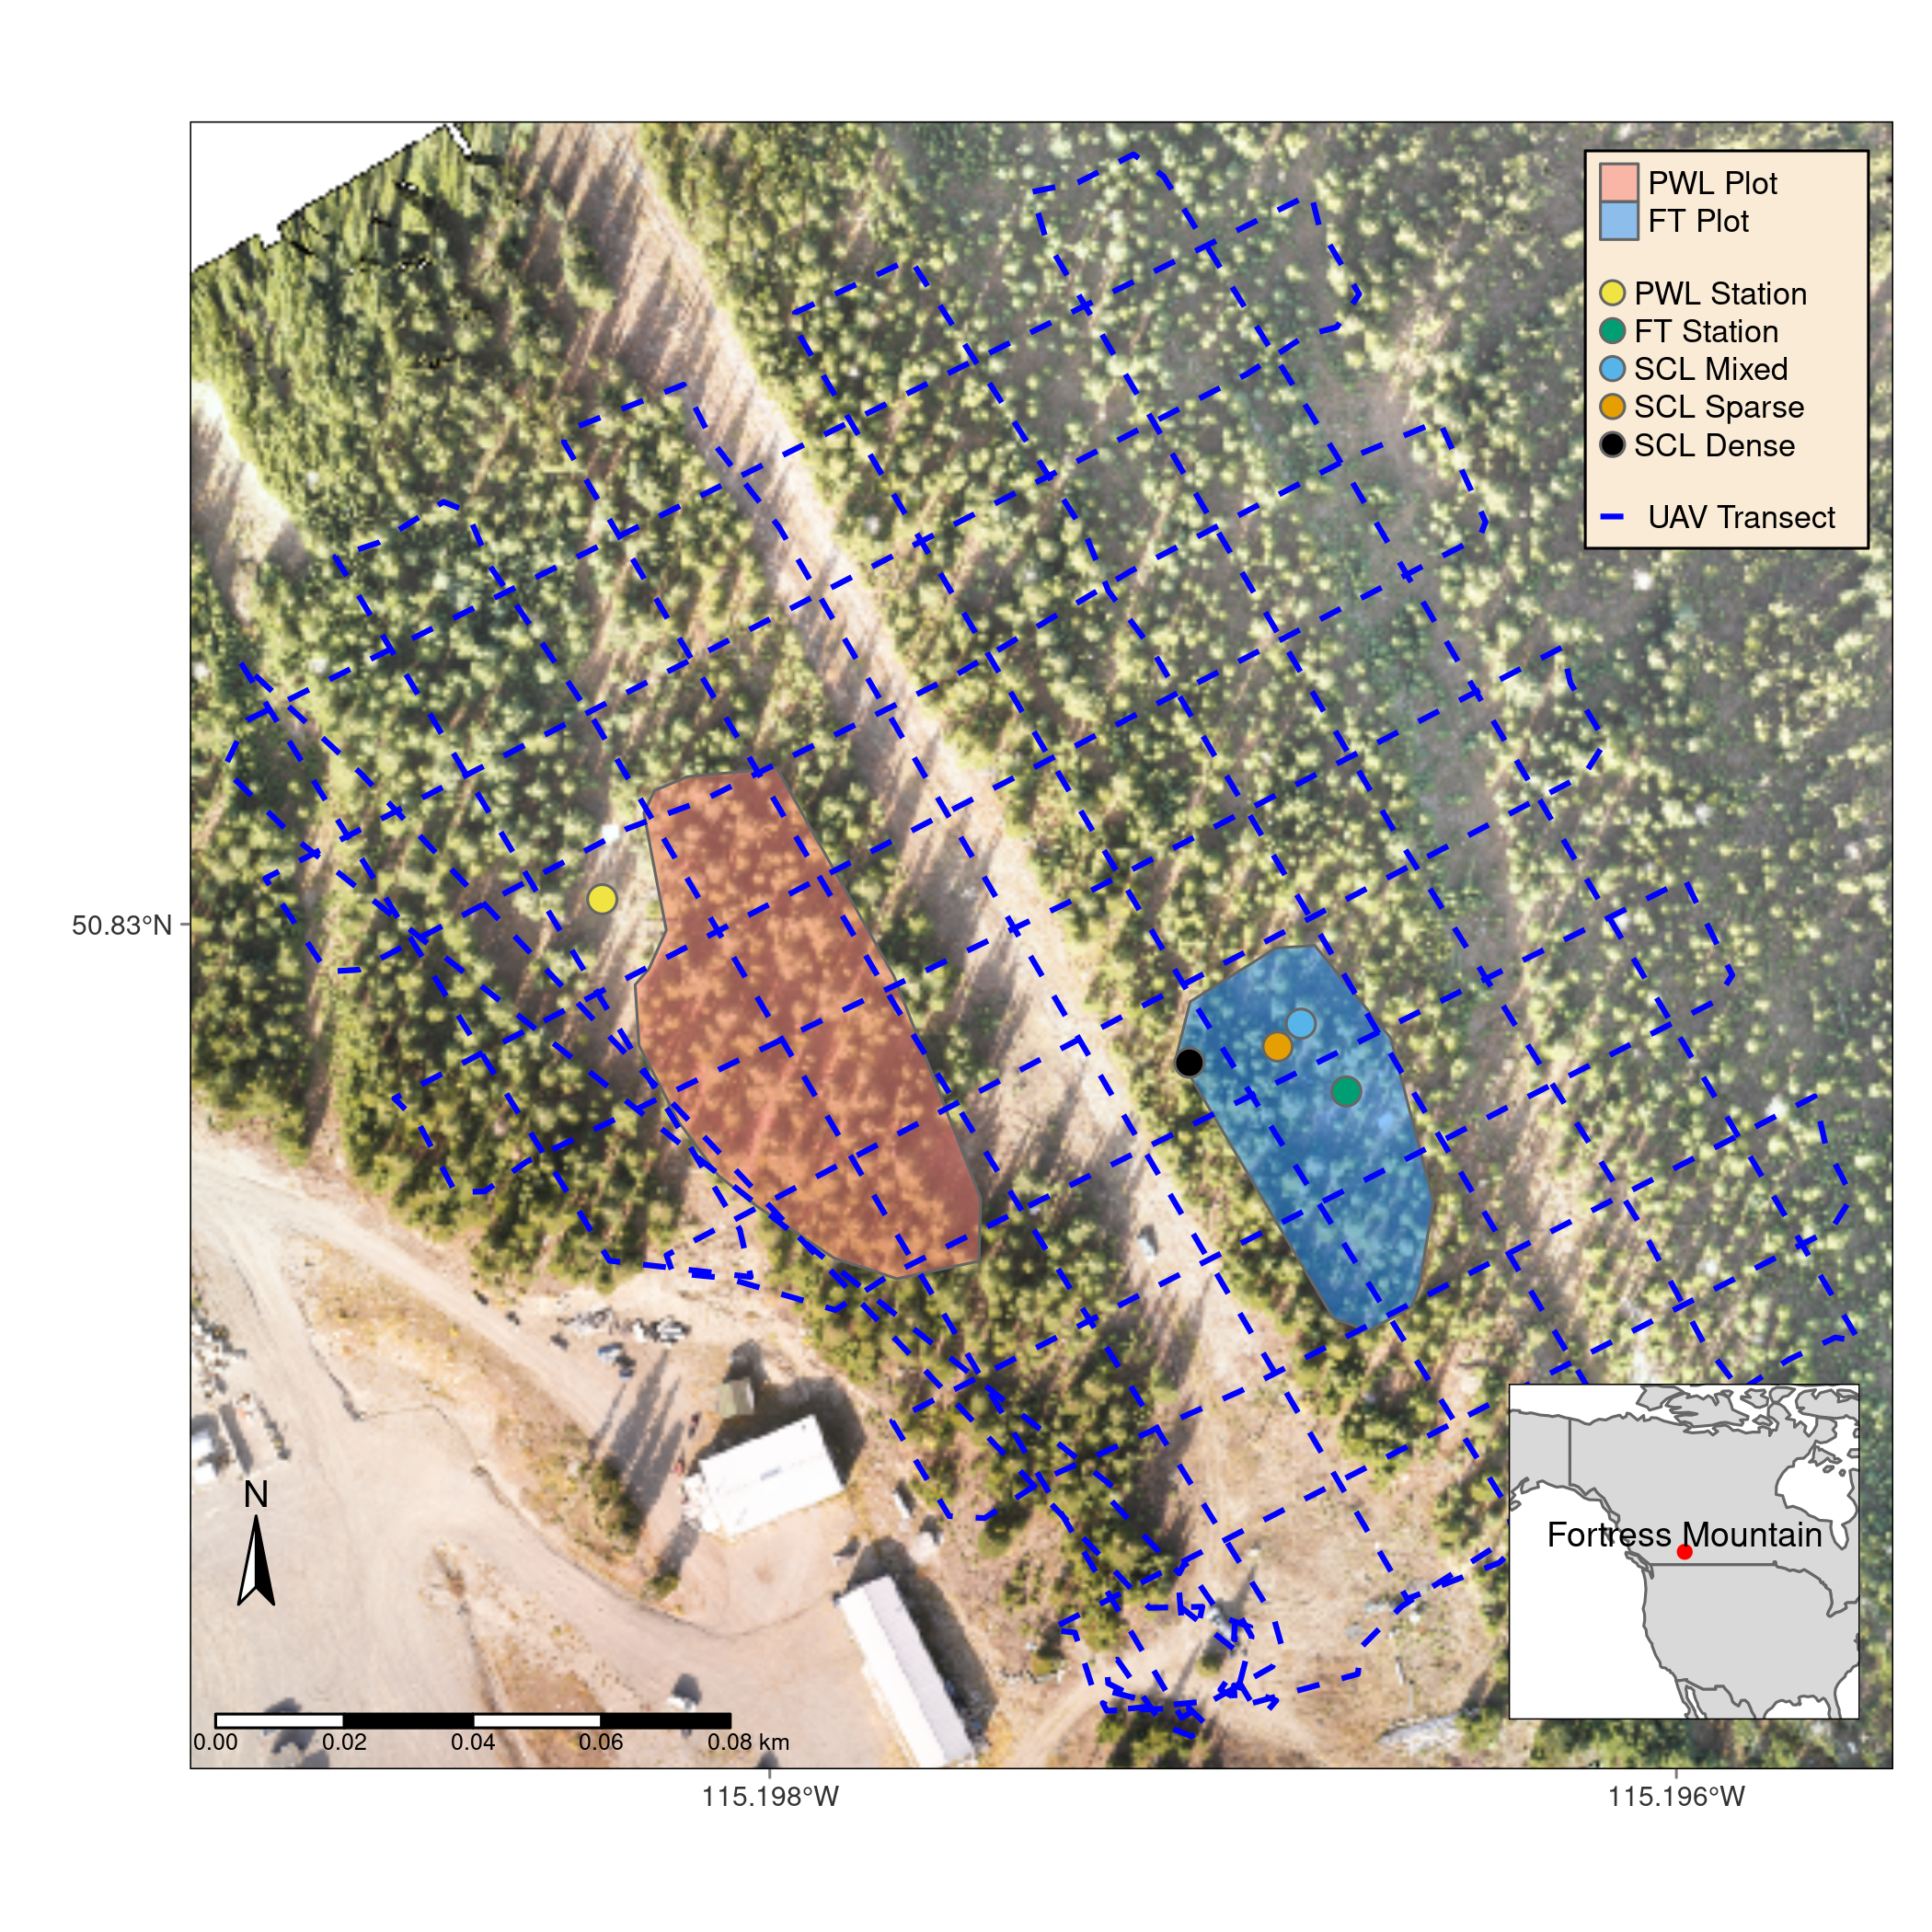
\includegraphics[keepaspectratio]{figs/study-site/site_map_inset.png}}

}

\caption{\label{fig-site-map}Map showing the location of forest plots,
flux towers, subcanopy lysimeter instruments, and survey transects. The
inset map on the lower right shows the regional location of Fortress
Mountain Research basin.}

\end{figure}%

\section{Methods}\label{methods}

\subsection{Statistics on Canopy Snow Unloading
Relationships}\label{statistics-on-canopy-snow-unloading-relationships}

\subsubsection{Combined influence of predictors on
unloading}\label{combined-influence-of-predictors-on-unloading}

The influence of air temperature, wind speed, snow load, melt, and
sublimation on the unloading process was assessed using a multivariate
ordinary least squares (OLS) regression. The analyses tested the
following hypotheses:

\begin{enumerate}
\def\labelenumi{\alph{enumi}.}
\tightlist
\item
  Melt promotes unloading through loss of structural integrity, particle
  bond weakening, and lubrication.
\item
  Sublimation promotes unloading via structural degradation and bond
  weakening.
\item
  Wind promotes unloading through shear stress on snow, wind erosion,
  and branch movement.
\item
  Air temperature promotes unloading by increased elasticity branches
  and association with melt/sublimation.
\end{enumerate}

Because many of these processes occur simultaneously and could not be
isolated experimentally, different combinations of the independent
variables were included in the regression to identify which sets of
processes significantly influenced unloading. The subcanopy lysimeter
unloading measurements had a high relative instrument error due to the
relatively small accumulation of unloaded snow over the 15-min
intervals. To improve instrument accuracy, while maintain consistency of
the unloading measurements with wind speed, the 15-min interval
measurements of unloading were aggregated over differing predictor
variable bins. Air temperature and wind speed were measured at FT
station, canopy snow load from the weighed tree lysimeter (scaled to the
canopy of each respective subcanopy lysimeter), and canopy snowmelt and
sublimation simulated in CRHM. Sublimation was simulated using
Equation~\ref{eq-ql} following Essery et al. (2003) and snowmelt
calculated using available energy from Equation~\ref{eq-eb} both
implemented in CRHM, were used for this analysis. Bins that had
accumulated unloaded snow less than 0.1 mm were removed which resulted
in a mean instrument error of +/- 2\% for the remaining bins. The
individual processes found to be significant predictors of unloading in
the multivariate regression (i.e., shear stress and canopy snow melt)
were then isolated to parameterise a model of their effects.

\subsubsection{Wind induced unloading}\label{wind-induced-unloading}

The influence of wind, shear stress and canopy snow load on unloading
was assessed during intervals without canopy snowmelt. These periods
were defined using simulated canopy snowmelt in CRHM and by visual
analysis of time-lapse imagery. By excluding periods influenced by melt,
the snow captured by the lysimeters is attributed primarily to
wind-driven unloading. Although unloading resulting from snow
metamorphism or thermally induced branch bending may also contribute,
the observed unloading is interpreted to be predominantly wind-induced
over these intervals. The relationship between wind speed, shear stress,
canopy snow load, and unloading was analyzed using linear and non-linear
least squares regression, with shear stress modeled linearly and wind
speed modeled exponentially.

\subsubsection{Canopy snowmelt induced
unloading}\label{canopy-snowmelt-induced-unloading}

A mass balance approach was incorporated to determine the unloading rate
resulting from canopy snowmelt (\(q_{unld}^{melt}\), mm
s\textsuperscript{-1}). The influence of canopy snowmelt on
\(q_{unld}^{melt}\) was then assessed by fitting a linear model using an
ordinary least squares regression. Since direct measurements of canopy
snow unloading are challenging to obtain independently from canopy
snowmelt drainage (Storck et al., 2002), the following mass balance was
incorporated to determine \(q_{unld}^{melt}\) as a residual:

\begin{equation}\phantomsection\label{eq-canopy-mass-bal}{
\frac{dL}{dt} = 
[q_{sf} - q_{tf} + q_{ros}] - [q_{unld}^{melt} + q_{unld}^{wind}] - q_{drip} - q_{wind}^{veg} - q_{sub}^{veg}
}\end{equation}

where \(\frac{dL}{dt}\) is the change in canopy snow load over time, (mm
s\textsuperscript{-1}), \(q_{sf}\) is the snowfall rate (mm
s\textsuperscript{-1}), \(q_{tf}\) (mm s\textsuperscript{-1}) is the
throughfall rate (mm s\textsuperscript{-1}), \(q_{ros}\) (mm
s\textsuperscript{-1}) is the rate of rainfall falling on snow
intercepted in the canopy, \(q_{unld}^{melt}\) is the canopy snow
unloading rate due to melt (mm s\textsuperscript{-1}),
\(q_{unld}^{wind}\) is the canopy snow unloading rate due to wind (mm
s\textsuperscript{-1}), \(q_{drip}\) is the canopy snow drip rate
resulting from canopy snowmelt (mm s\textsuperscript{-1}),
\(q_{wind}^{veg}\) is the wind transport rate in or out of the control
volume (mm s\textsuperscript{-1}), and \(q_{sub}^{veg}\) is the
intercepted snow sublimation rate (mm s\textsuperscript{-1}). Figure 1
in Cebulski \& Pomeroy (2025b) presents a visual representation of this
mass balance. Little research has examined the the water-holding
capacity of snow intercepted in the canopy; however in this study it is
assumed to be minimal such that \(q_{drip} \approx q_{melt}\).

Then Equation~\ref{eq-canopy-mass-bal} was rearranged to solve for
\(q_{unld}^{melt}\) during intervals without
\([q_{sf} - q_{tf} + q_{ros}]\) or \(q_{wind}^{veg}\) as:

\begin{equation}\phantomsection\label{eq-unld-melt-mass-bal}{
q_{unld}^{melt} = -\frac{dL}{dt} - q_{drip} - q_{unld}^{wind} - q_{sub}^{veg}
}\end{equation}

While some components of the canopy snow mass balance can be measured
directly with relative ease, such as \(\frac{\Delta L}{\Delta t}\) with
the weighed tree, sublimation of canopy snow is more difficult to
quantify directly especially in forested mountain environments (Conway
et al., 2018; Helgason \& Pomeroy, 2012b) and thus \(q_{sub}^{veg}\) was
simulated in this study in CRHM using Equation~\ref{eq-ql} as described
in Essery et al. (2003). \(q_{drip}\) was measured where possible using
the tipping buckets, however problems with freezing of liquid water in
the devices limited the amount of \(q_{drip}\) that could be collected.
Thus, \(q_{drip}\) was also supplemented with simulated canopy snowmelt
(\(q_{melt}\)) in CRHM as in Equation~\ref{eq-eb}. Canopy snow ablation
periods that were dominated by melt were selected for calculating
\(q_{unld}^{melt}\) where the contribution of \(q_{unld}^{wind}\) and
\(q_{sub}^{veg}\) to canopy snow ablation was less than 5\%.

\section{Canopy Snow Energy Balance}\label{canopy-snow-energy-balance}

A revised canopy snow energy balance is presented here which provided
both an approximation of canopy snowmelt and sublimation as these
processes could not be measured directly and also for use in the canopy
snow ablation routines. The energy available for melting snow
intercepted in the canopy, \(Q_{melt}\) (W m\textsuperscript{-2}), which
is a function of the canopy snow load (\(L\)) was calculated as:

\begin{equation}\phantomsection\label{eq-eb}{
Q_{melt}(L) = 
Q_{sw} +
Q_{lw} +
Q_{p} + Q_{h} + Q_{l} - [C_p^{ice} L \frac{\Delta T_{vs}}{\Delta t}]
}\end{equation}

where \(Q_{sw}\) and \(Q_{lw}\) (W m\textsuperscript{-2}) are the net
shortwave and longwave radiation heat fluxes to the canopy snow, \(Q_p\)
(W m\textsuperscript{-2}), is the advective energy rate, and \(Q_{l}\)
and \(Q_{h}\) (W m\textsuperscript{-2}), are the turbulent fluxes of
latent heat and sensible heat respectively (positive towards canopy
snow), \(C_p^{ice}\) (J kg\textsuperscript{-1} K\textsuperscript{-1}) is
the specific heat capacity of ice, and
\(\frac{\Delta T_{vs}}{\Delta t}\) (K s\textsuperscript{-1}) is the
change in canopy snow temperature over time.

\(Q_{sw}\) was determined as:

\begin{equation}\phantomsection\label{eq-sw}{
Q_{sw} = \downarrow Q_{sw} \cdot (1 - \alpha_s) \cdot \tau_{50}^{veg}
}\end{equation}

where \(\downarrow Q_{sw}\) is the downwelling shortwave radiation (W
m\textsuperscript{-2}), \(\alpha_s\) is the albedo of snow intercepted
in the canopy (-), \(\tau_{50}^{veg}\) (-) is the canopy transmittance
to \(\downarrow Q_{sw}\). \(\tau_{50}^{veg}\) was determined using
Equation from Pomeroy et al. (2009) with half of the leaf area index
(LAI), following studies (Kesselring et al., 2024; Weiskittel et al.,
2009), who report that approximately 50\% of the total leaf area is
concentrated in the upper half of coniferous canopies. This provides an
approximation of the mean \(Q_{sw}\) to all snow intercepted in the
canopy, and is a simplification from using a partial differential
equation to determine the radiation incident to individual height layers
within the canopy. Upwelling shortwave radiation reflected off of the
surface snowpack is considered negligible contribution to the snow
intercepted in the canopy as it is primarily blocked by vegetation
elements underlying the canopy snow.

\(Q_{lw}\) was approximated as:

\begin{equation}\phantomsection\label{eq-lw}{
Q_{lw} = \downarrow Q_{lw}^{atm} + \uparrow Q_{lw}^{veg} + \uparrow Q_{lw}^{veg2veg} - Q_{lw}^{vs}
}\end{equation}

where \(Q_{lw}^{atm}\) is the downwelling longwave radiation from the
atmosphere (W m\textsuperscript{-2}), \(Q_{lw}^{veg}\) is the longwave
radiation upwelling from vegetation elements underlying snow intercepted
in the canopy (W m\textsuperscript{-2}), \(Q_{lw}^{veg2veg}\) is the
downwelling longwave radiation emitted from the underside of the
vegetation elements reflected by the subcanopy snowpack (W
m\textsuperscript{-2}), and \(Q_{lw}^{vs}\) (W m\textsuperscript{-2}) is
the outgoing longwave radiation from the top and bottom of the canopy
snow layer calculated as:

\begin{equation}\phantomsection\label{eq-lw-vs}{
Q_{lw}^{vs} = 2 \epsilon_{s} \sigma T_{vs}^4
}\end{equation}

where \(\epsilon_s\) is the emissivity (-) of snow taken as 0.99 and
\(\sigma\) is the Stefan--Boltzmann (5.67e-10 W m\textsuperscript{-1}
K\textsuperscript{-4}). \(Q_{lw}^{atm}\) was approximated in this study
as in Sicart et al. (2006) to take into account the influence of
atmospheric moisture on emissivity. \(Q_{lw}^{veg}\) was calculated with
the assumption that canopy elements were in equilibrium with the air
temperature plus any change in vegetation temperature from the
extinction of \(\downarrow Q_{sw}\) in the canopy (Pomeroy et al., 2009,
Eq. 4).

\(Q_p\) was calculated as:

\begin{equation}\phantomsection\label{eq-qp}{
Q_p = [C_p^{wtr} m_r(T_r - T_{vs}) + C_p^{ice} m_s(T_s - T_{vs})] / \Delta t
}\end{equation}

where \(C_p^{wtr}\) is the specific heat capacity of water (J
kg\textsuperscript{-1} K\textsuperscript{-1}), \(m_r\) is the specific
mass of liquid water in precipitation (mm), \(T_r\) is the rainfall
temperature (K), \(m_s\) is the specific mass of snow in precipitation
(mm), and \(T_s\) is the snowfall temperature (K).

\(Q_h\) was calculated as:

\begin{equation}\phantomsection\label{eq-qh}{
Q_h = \frac{\rho_a}{r_a} C_p^{air} (T_a - T_{vs})
}\end{equation}

where \(\rho_a\) is the air density (kg m\textsuperscript{-3}),
\(C_p^{air}\) is the specific heat capacity of air (J
kg\textsuperscript{-1} K\textsuperscript{-1}), \(T_a\) is the air
temperature, and \(r_a\) is the aerodynamic resistance (s
m\textsuperscript{-1}) which was approximated from Equation 4 from Allan
et al. (1998) as:

\begin{equation}\phantomsection\label{eq-ra}{
r_a = \frac{\text{log}(\frac{z_T - d_0}{z_0})\text{log}(\frac{z_u - d_0}{z_0})}{\kappa^2 u_z}
}\end{equation}

where \(z_T\) is the height of temperature measurement (m), \(d_0\) is
the displacement height (m) which was approximated as
2/3\textsuperscript{rd} the mean canopy height, \(z_0\) is the roughness
length (m) which was approximated as 1/10\textsuperscript{th} of the
mean canopy height, \(z_u\) is the wind speed measurement height (m),
\(\kappa\) is von Karman's constant, 0.41 (-), and \(u_z\) is the wind
speed measurement at \(z_u\) (m s\textsuperscript{-1}).

\(Q_l\) was calculated as:

\begin{equation}\phantomsection\label{eq-ql}{
Q_l = \frac{\rho_a}{r_i+r_a} (q_a(T_a) - q_{vs}(T_{vs}))
}\end{equation}

where \(r_i\) is a resistance for transport of moisture from intercepted
snow to the canopy air space (Eq. 28 in Essery et al., 2003),
\(q_a(T_a)\) and \(q_{vs}(T_{vs})\) are the specific humidity (-) at the
air temperature and canopy snow temperature respectively. If the height
of the air temperature measurement differs from the humidity measurement
the \(z_T\) term in the Equation~\ref{eq-ra} should be adjusted to use
the the humidity measurement height.

The above sensible and latent heat flux equations assume neutral
atmospheric stability conditions, i.e., nearly adiabatic conditions (no
heat exchange) which may be appropriate for application with snow which
is intercepted in the roughness elements where stability corrections may
not be required (Allan et al., 1998). This is also supported by the
uncertainty of stability correction in forest canopies (Conway et al.,
2018) and mountain environments (Helgason \& Pomeroy, 2012a). Solving
Equation~\ref{eq-eb} requires an iterative solution to determine
\(\Delta T_{vs}\) and the remaining terms which are also a function of
\(T_{vs}\).

\section{Modelled Canopy Snow Energy and Mass
Balance}\label{modelled-canopy-snow-energy-and-mass-balance}

The energy and mass balance of canopy snow was simulated using the Cold
Regions Hydrological Model (CRHM) to evaluate the new canopy snow
ablation routine. A full description of the CRHM model is described in
Pomeroy et al. (2007) and the up to date source code is available at
https://github.com/srlabUsask/crhmcode. In addition to the updated
parameterizations presented in this study, parameterizations from
previous studies that simulate canopy snow unloading, melt, and
sublimation were also implemented and compared against the updated
routine within CRHM. Canopy snow sublimation simulations also provided
the rate of sublimation needed in Equation~\ref{eq-unld-melt-mass-bal}.

In addition to the updated parameterizations presented in this study,
three other canopy snow routines were implemented in CRHM following
previous studies by Ellis et al. (2010) and Floyd (2012) (hereafter
Ellis2010), Roesch et al. (2001) (Roesch2001), and Andreadis et al.
(2009) (Andreadis2009). The Ellis et al. (2010) routine was previously
integrated into CRHM as a module and is the one typically used to
simulated snow accumulation in forests in CRHM and was run as is. The
Ellis2010 module includes canopy snow sublimation as described in
Pomeroy et al. (1998), canopy snow unloading over time from Hedstrom \&
Pomeroy (1998) with modifications described in Floyd (2012) to handle
canopy snow melt and drip processes using an ice-bulb temperature
threshold. The Roesch2001 routine represents canopy snow unloading and
melt using wind and air temperature functions. The Andreadis2009
parameterization unloads snow as a function of canopy snowmelt alone,
following observations by Storck et al. (2002) and does not include wind
induced unloading. The snowmelt rate from Equation~\ref{eq-eb} was used
to calculate the unloading rate for the Andreadis2009 unloading. The
default parameters provided by each individual study were used here and
were not calibrated. More details on the aforementioned
parameterizations are described in Cebulski \& Pomeroy (2025b).

\section{Results}\label{results}

\subsection{Canopy Snow Unloading
Relationships}\label{canopy-snow-unloading-relationships}

A positive relationship (\emph{p} \textless{} 0.05,
\emph{R\textsuperscript{2}} = 0.79) was identified between canopy load,
canopy snowmelt, wind speed, and the rate of canopy snow unloading, as
measured by the subcanopy lysimeters. This set of predictors yielded the
highest \emph{R\textsuperscript{2}} among the models tested
(Table~\ref{tbl-q-unld-bins}). Shear stress was found to explain less
variability compared to wind speed, when combined with canopy snow load
and snowmelt (\emph{p} \textless{} 0.05, \emph{R\textsuperscript{2}} =
0.71). Air temperature and canopy snow sublimation were not significant
predictors in any model (\emph{p} \textgreater{} 0.05;
Table~\ref{tbl-q-unld-bins}). A model including only canopy load, air
temperature, and wind speed produced an \emph{R\textsuperscript{2}} of
0.11, though only canopy load and wind speed were statistically
significant (\emph{p} \textless{} 0.05). As shown in
Fig.~\ref{fig-q-unld-all-bins}, unloading rates were substantially more
variable across the canopy snowmelt and sublimation bins (0--2 mm
hr\textsuperscript{-1}) compared to the air temperature and wind speed
bins (0--0.5 mm hr\textsuperscript{-1}). As a result, models without
canopy snowmelt explained substantially less variation in unloading.
Additional model comparisons with various combinations of independent
variables are presented in the supporting information.

The mean unloading rate was observed in Fig.~\ref{fig-q-unld-all-bins}
to increase with increasing canopy load, air temperature, ice-bulb
temperature depression, shear stress, and wind speed. Despite the
insignificant relationships, air temperature and canopy snow sublimation
were positively associated with canopy snow unloading, though for
sublimation this relationship was limited to sublimation rates between 0
and 0.3 mm hr\textsuperscript{-1} (Fig.~\ref{fig-q-unld-all-bins}). For
sublimation rates higher than 0.3 hr\textsuperscript{-1}, unloading is
observed to decline with increasing sublimation, as more canopy snow is
partitioned to the atmosphere. A decline in unloading is observed for
wind speed bins above 3 m s\textsuperscript{-1} which is attributed to
some wind transport of canopy snow, and potential entrainment into the
atmosphere, and corresponding increased sublimation rates.

\begin{longtable}[]{@{}
  >{\raggedright\arraybackslash}p{(\linewidth - 18\tabcolsep) * \real{0.1146}}
  >{\raggedright\arraybackslash}p{(\linewidth - 18\tabcolsep) * \real{0.1146}}
  >{\raggedright\arraybackslash}p{(\linewidth - 18\tabcolsep) * \real{0.1042}}
  >{\raggedright\arraybackslash}p{(\linewidth - 18\tabcolsep) * \real{0.1146}}
  >{\raggedright\arraybackslash}p{(\linewidth - 18\tabcolsep) * \real{0.1146}}
  >{\raggedright\arraybackslash}p{(\linewidth - 18\tabcolsep) * \real{0.1146}}
  >{\raggedright\arraybackslash}p{(\linewidth - 18\tabcolsep) * \real{0.0938}}
  >{\raggedright\arraybackslash}p{(\linewidth - 18\tabcolsep) * \real{0.1042}}
  >{\raggedleft\arraybackslash}p{(\linewidth - 18\tabcolsep) * \real{0.0625}}
  >{\raggedleft\arraybackslash}p{(\linewidth - 18\tabcolsep) * \real{0.0625}}@{}}

\caption{\label{tbl-q-unld-bins}Summary of multiple linear regression
results evaluating all combinations of predictor variables for canopy
snow unloading including: canopy load (\(L\)), wind speed (\(u\)),
canopy snowmelt rate (\(q_{melt}\)), canopy snow sublimation rate
(\(q_{subl}\)), and air temperature (\(T_a\)). Columns L to Ta show the
coefficient estimate for each respective term, and the significance of
each term is shown in brackets. Significance codes: * = p \textless{}
0.05; ns = not significant (p \textgreater{} 0.05). The models are
ranked by their corresponding AIC value.}

\tabularnewline

\toprule\noalign{}
\begin{minipage}[b]{\linewidth}\raggedright
Model Name
\end{minipage} & \begin{minipage}[b]{\linewidth}\raggedright
Intercept
\end{minipage} & \begin{minipage}[b]{\linewidth}\raggedright
\(L\)
\end{minipage} & \begin{minipage}[b]{\linewidth}\raggedright
\(u\)
\end{minipage} & \begin{minipage}[b]{\linewidth}\raggedright
\(q_{melt}\)
\end{minipage} & \begin{minipage}[b]{\linewidth}\raggedright
\(q_{subl}\)
\end{minipage} & \begin{minipage}[b]{\linewidth}\raggedright
\(\tau\)
\end{minipage} & \begin{minipage}[b]{\linewidth}\raggedright
\(T_a\)
\end{minipage} & \begin{minipage}[b]{\linewidth}\raggedleft
\(R^2\)
\end{minipage} & \begin{minipage}[b]{\linewidth}\raggedleft
AIC
\end{minipage} \\
\midrule\noalign{}
\endhead
\bottomrule\noalign{}
\endlastfoot
M1 & -0.11 (ns) & 0.02 (*) & 0.08 (*) & 0.40 (*) & --- & --- & --- &
0.79 & -12.8 \\
M4 & -0.08 (ns) & 0.04 (*) & --- & 0.39 (*) & --- & 0.75 (*) & --- &
0.71 & 5.5 \\
M7 & 0.13 (ns) & 0.02 (*) & --- & 0.32 (*) & -0.22 (ns) & --- & --- &
0.54 & 10.0 \\
M10 & -0.06 (ns) & 0.02 (*) & 0.08 (*) & 0.38 (*) & --- & --- & 0.00
(ns) & 0.52 & -4.4 \\
M24 & -0.00 (ns) & 0.02 (*) & 0.05 (*) & 0.36 (*) & 0.13 (ns) & --- &
--- & 0.37 & -2.0 \\
M40 & 0.07 (ns) & 0.01 (*) & 0.06 (*) & --- & --- & --- & 0.01 (ns) &
0.11 & 2.4 \\
M63 & 0.22 (*) & 0.00 (ns) & -0.01 (ns) & --- & 0.07 (ns) & --- & --- &
-0.02 & 39.8 \\

\end{longtable}

\begin{figure}[H]

\centering{

\pandocbounded{\includegraphics[keepaspectratio]{figs/results/explore/scl_q_unld_vs_bins.png}}

}

\caption{\label{fig-q-unld-all-bins}Scatter plots showing the mean
canopy snow unloading rate for differing bins of air temperature (°C),
ice-bulb temperature depression (°C), shear stress (N
m\textsuperscript{-2}), canopy snowmelt (mm hr\textsuperscript{-1}),
canopy snow sublimation (mm hr\textsuperscript{-1}), and wind speed (m
s\textsuperscript{-1}). Note: canopy snow unloading was measured by the
subcanopy lysimeters, air temperature and wind speed were measured at FT
station, canopy snowmelt and sublimation were modelled in CRHM.}

\end{figure}%

\subsubsection{Wind Induced Unloading}\label{wind-induced-unloading-1}

Canopy snow unloading measurements from the subcanopy lysimeters,
filtered to include intervals without canopy snowmelt, followed a
positive linear relationship with shear stress and a positive
exponential relationship with wind speed (Fig.~\ref{fig-q-unld-wind}).
Based on these observed relationships the following relationships were
fit and tested against the observed data:

The wind-driven canopy snow unloading rate, \(q_{unld}^{wind}\), was
represented as a linear function of shear stress:

\begin{equation}\phantomsection\label{eq-q-unld-tau}{
q_{unld}^{wind} = L \cdot \tau_{mid} \cdot a
}\end{equation}

where \(\tau_{mid}\) is the shear stress at mid canopy height and \(a\)
is a fitting constant.

An exponential function of wind speed was defined as:

\begin{equation}\phantomsection\label{eq-q-unld-wind}{
q_{unld}^{wind} = L \cdot u_{mid} \cdot a \cdot e^{b\cdot u_{mid}}
}\end{equation}

where \(u_{mid}\) is the wind speed at mid canopy height, and \(a\) and
\(b\) are fitting constants.

The shear stress relationship (Equation~\ref{eq-q-unld-tau}) accounted
for slightly more variability in unloading (\emph{p} \textless{} 0.05,
\emph{R\textsuperscript{2}} = 0.61), likely due to its better relation
to the kinetic energy required to unload snow compared to wind speed
(\emph{p} \textless{} 0.05, \emph{R\textsuperscript{2}} = 0.54). The
mean bias of the shear stress model of 0.037 mm hr\textsuperscript{-1}
is also lower compared to the wind speed model of 0.048 mm
hr\textsuperscript{-1}, additional model error statistics and fitting
coefficients are provided in Table~\ref{tbl-q-unld-wind}. Both models
exhibited considerable scatter across the different bins, with notable
uncertainty within each bin (Fig.~\ref{fig-q-unld-wind}). The
wind-induced unloading rate was observed to be higher for bins with
higher canopy snow load across nearly all bins
(Fig.~\ref{fig-q-unld-wind}). The \emph{R\textsuperscript{2}} of both
the shear stress and wind speed relationships is much higher than the
amount of variance explained by wind speed when including intervals with
melting snow (Table~\ref{tbl-q-unld-bins}). The increased liquid water
content during the canopy snowmelt process may provide some resistance
to wind induced unloading. However, a statistically significant negative
influence of air temperature on wind speed could not be found, likely
due to the strong positive association of air temperature and melt on
unloading. Moreover, increased canopy snow unloading during low wind
speeds, resulting from high melt rates could also contribute to the
lower explanatory power of wind speed in Table~\ref{tbl-q-unld-bins}.
The higher \emph{R\textsuperscript{2}} of the shear stress model
compared to wind speed, coupled with the better phyical representation
of kinetic energy, provided the reasoning for selecting shear stress as
the independent variable to predict wind-induced unloading.

\begin{figure}[H]

\centering{

\pandocbounded{\includegraphics[keepaspectratio]{figs/results/modelled_tau_wind_unloading_w_obs.png}}

}

\caption{\label{fig-q-unld-wind}Canopy snow unloading rate measured by
the subcanopy lysimeters versus shear stress (left) and wind speed
(right) during periods without canopy snowmelt. The dots represent mean
unloading rates within bins of shear stress and wind speed; error bars
indicate +/- 1 standard deviation. The fitted lines show predictions
from Equation~\ref{eq-q-unld-tau} (left) and
Equation~\ref{eq-q-unld-wind} (right).}

\end{figure}%

\begin{longtable}[]{@{}lll@{}}

\caption{\label{tbl-q-unld-wind}Summary of the performance and
regression coefficients for the relationship between canopy snow
unloading with wind speed (Equation~\ref{eq-q-unld-tau}) and shear
stress (Equation~\ref{eq-q-unld-wind}), as shown in
Fig.~\ref{fig-q-unld-wind}. Coefficients are developed for hourly
unloading.}

\tabularnewline

\toprule\noalign{}
Metric & Wind & Shear Stress \\
\midrule\noalign{}
\endhead
\bottomrule\noalign{}
\endlastfoot
Mean Bias (mm/hr) & 0.048 & 0.037 \\
Mean Absolute Error (mm/hr) & 0.087 & 0.115 \\
Root Mean Square Error (mm/hr) & 0.11 & 0.15 \\
Coefficient of Determination (\(R^2\)) & 0.54 & 0.61 \\
Coefficient a & 4.62e-03 & 3.31e-01 \\
Significance of a & p \textless{} 0.05 & p \textless{} 0.05 \\
Coefficient b & 3.93e-01 & NA \\
Significance of b & p \textless{} 0.05 & NA \\

\end{longtable}

\subsubsection{Melt induced unloading}\label{melt-induced-unloading}

A positive linear relationship was identified between the ratio of
canopy snow unloading to melt and canopy snow load
(Fig.~\ref{fig-unld-melt-ratio}). This ratio ranged from approximately
0--0.5 for snow loads between 0 and 5 mm, and increased to a maximum of
5 at a canopy snow load of 30 mm (Fig.~\ref{fig-unld-melt-ratio}). This
relationship was represented by the following equation:

\begin{equation}\phantomsection\label{eq-q-unld-melt}{
q_{unld}^{melt} = f(m) \cdot q_{melt}(L)
}\end{equation}

where \(f(m)\) is the ratio of unloading to canopy snowmelt and
\(q_{melt}\) is the canopy snowmelt rate (mm hr\textsuperscript{-1}).
Equation~\ref{eq-q-unld-melt} is similar to Equation 33 in Andreadis et
al. (2009); however, instead of assuming a constant value of 0.4 for
\(f(m)\), it was determined as:

\begin{equation}\phantomsection\label{eq-fm}{
f(m) = m \cdot L + b
}\end{equation}

where \(m\) and \(b\) were determined as 0.16 and -0.5, respectively,
using an ordinary least squares regression.

Equation~\ref{eq-q-unld-melt} resulted in a statistically significant
relationship (\emph{p} \textless{} 0.05, \emph{R\textsuperscript{2}} =
0.73) for canopy snow ablation events in which wind-driven unloading
and/or sublimation contributed less than 5\% to total ablation less than
5\%, based on ordinary least squares linear regression
(Fig.~\ref{fig-unld-melt-ratio}). The regression was performed using the
data shown in Fig.~\ref{fig-unld-melt-ratio}, which presents the ratio
of canopy snow unloading, derived from the weighed tree using
Equation~\ref{eq-unld-melt-mass-bal} using simulated \(q_{melt}\).
Additional observations of canopy snowmelt melt from the tipping buckets
were also used to compute the canopy snow unloading-to-melt ratio
(Fig.~\ref{fig-unld-melt-ratio}); however, the number of usable
observations was limited due to freeze-thaw events that affected the
instrument functionality. These measurements are still useful in
providing some indication of the validity of the CRHM canopy
snowmelt/drip routine (Fig.~\ref{fig-obs-mod-cpy-load-mb}). The CRHM
estimated cumultive drip is higher than the tipping buckets for two out
of the three melt events. A difference in the timing and magnitude of
the observed and simulated values were expected due to both instrument
uncertainties in the tipping buckets (freezing/thawing) and in the
canopy snow energy balance simulation.

\begin{figure}[H]

\centering{

\pandocbounded{\includegraphics[keepaspectratio]{figs/results/modelled_melt_unloading_ratio_vs_snow_load_bin.png}}

}

\caption{\label{fig-unld-melt-ratio}The ratio of canopy snow unloading
(weighed tree residual) to snowmelt across different canopy snow load
bins and events. Black dots represent the observed cumulative unloading
divided by the cumulative simulated snowmelt from CRHM. Red dots show
the cumulative observed unloading divided by snowmelt measured by the
tipping buckets. Multiple dots within a bin correspond to different
events. The blue line represents the best-fit line derived from ordinary
least squares regression.}

\end{figure}%

\begin{figure}[H]

\centering{

\includegraphics[width=0.85\linewidth,height=\textheight,keepaspectratio]{figs/results/crhm_vs_tb_drip_events_2025-05-09-10-30-14_ffr_closed_canopy_cc0.88_cansnobal_cansnobal_v_3_0_w_asm_output.png}

}

\caption{\label{fig-obs-mod-cpy-load-mb}Cumulative canopy snow drip from
the mean of the tipping buckets (TB\_mean) and the updated canopy
snowmelt routine (crhm\_drip).}

\end{figure}%

\subsection{Evaluation of canopy snow ablation
parameterisations}\label{evaluation-of-canopy-snow-ablation-parameterisations}

The updated canopy snow ablation routine which includes canopy snowmelt
estimated from the energy balance described by Equation~\ref{eq-eb},
sublimation rate from Equation~\ref{eq-ql}, wind-driven unloading using
Equation~\ref{eq-q-unld-tau}, and melt induced unloading from
Equation~\ref{eq-q-unld-melt} was assessed against observed canopy snow
ablation from the weighed tree across 17 post-snowfall periods. These
ablation periods had air temperatures ranging from -30.5°C to 6.9°C and
wind speeds from calm to 5.3 m s\textsuperscript{-1}
(Table~\ref{tbl-event-met}). The contribution of canopy snowmelt (and
associated unloading), sublimation, and wind-driven unloading was used
to classify individual events as either melt, sublimation, wind, or
mixed (combination of many processes) dominated
(Fig.~\ref{fig-sim-frac-abl}). Melt dominated events had a fraction of
over 0.85 of total ablation and had the least contribution from wind and
sublimation (0 to 0.13). Sublimation and wind dominated events had
minimal contribution of melt but due to the correlation of these two
processes were difficult to isolate from one another.

The observed and simulated canopy snow load over each of the ablation
events is shown in Fig.~\ref{fig-obs-mod-w-tree}. When averaged over all
events the updated routine resulted in a reduced mean bias of 0.04 mm
hr\textsuperscript{-1} compared to existing models which had a mean
biases ranging from 0.06 to 0.12 mm hr\textsuperscript{-1} when assessed
with hourly weighed tree ablation and averaged across all events
(Table~\ref{tbl-obs-mod-stats-avg}). For the melt-dominated events, the
two parameterizations that include an energy balance based routine track
the observed decline in snow load over the melt process well in
Fig.~\ref{fig-obs-mod-w-tree} with mean biases in hourly ablation of
-0.03 mm hr\textsuperscript{-1} and -0.06 mm hr\textsuperscript{-1} for
the new and Andreadis2009 routine respectively and a small range in mean
biases across the differing melt events
(Fig.~\ref{fig-obs-mod-cpy-load-mb}). The air temperature (roesch2001)
and ice-bulb temperature (Ellis2010) based routines have less
consistency over these events (Fig.~\ref{fig-obs-mod-cpy-load-mb})
resulting in mean biases of 0.28 to 0.41 mm hr\textsuperscript{-1}. The
slight improvement for the updated routine compared to Andreadis2009
comes from the better representation of the increase in unloading for
higher canopy snow loads (Equation~\ref{eq-fm}) as observed for the
2022-06-14 event which had much higher snow load of 30 mm.

A small improvement in the mean bias over all events was observed for
sublimation events in the updated routine, of -0.02 mm
hr\textsuperscript{-1} compared to the other models which ranged from
-0.04 to NA mm hr\textsuperscript{-1}
(Table~\ref{tbl-obs-mod-stats-avg}). The ellis2010 and andreadis2009
parameterizations resulted in a larger range in mean biases across the
events (Fig.~\ref{fig-obs-mod-cpy-load-mb}) particularly during
clear-sky nights, which led to cooling of the canopy snow surface
temperature and thus supression of the canopy snow sublimation rate.
This effect could be represented in the Essery et al. (2003) energy
balance based routine but not in the Pomeroy et al. (1998) routine,
which assumes that the canopy snow surface temperature remains in
thermoequilibrium with the air temperature
(Fig.~\ref{fig-obs-mod-w-tree}). See event `2022-03-24' in
Fig.~\ref{fig-obs-mod-w-tree} for an example of this where the rate of
sublimation slows at night an better matches the observation compared to
the other models (and 2022-03-14 to a lesser extent). For relatively
warm sublimation events, i.e., 2022-03-02 the ellis2010 and roesch2001
parameterizations over estimate ablation as they start to melt and
unload snow from the canopy rapidly, while the energy balance method
better captures the cooling effect of sublimation which suppresses the
melt process (although the air temperature is above 0°C). Still some
variability is observed with the energy balance based routines where the
magnitude of ablation is over estimated for the 2023-03-14 event for the
new routine, likely due to over estimation of wind induced unloading (on
average), the timing of sublimation by the andreadis2009 routine is good
here but it does not include wind unloading at all so misses the steep
decline in canopy snow during specific wind periods the Ellis2010
routine over estimates total ablation here as well due to over
estimation of sublimation at night due to night time cooling effects and
inclusion of time induced unloading.

The wind-driven unloading events show the importance of representing
this process, with models that simulate wind-induced unloading having
lower mean bias of 0.21 mm hr\textsuperscript{-1} for the Roesch et al.
(2001) linear model and 0.29 mm hr\textsuperscript{-1} in the updated
model, compared to the mean bias of over 0.57 mm hr\textsuperscript{-1}
for the two simulations that do not directly incorporate wind-induced
unloading (Table~\ref{tbl-obs-mod-stats-avg}). The roesch2001
parameterization over estimates the mean event unloading for two of the
events, the updated routine is slightly more stable across the differing
events, but still understimates mean event for event 2023-02-24 which
has peak wind speeds of over 5 m s\textsuperscript{-1} and potentially
some amount of wind transport process which is not directly accounted
for. The wind induced unloading process resulted in the overall mean
bias compared to the melt and sublimation dominated events, even
compared to the wind unloading function developed at the same site (from
the subcanopy lysimeters).

\pagebreak
\setstretch{1.0}

\begin{table}

\caption{\label{tbl-event-met}Meteorology of the 17 select ablation
events. Air temperature, relative humidity, and wind speed were measured
at FT station. The process fractions show the fraction of canopy snow
ablation for each process.}

\centering{

\fontsize{12.0pt}{14.4pt}\selectfont
\begin{tabular*}{\linewidth}{@{\extracolsep{\fill}}>{\centering\arraybackslash}p{\dimexpr 67.50pt -2\tabcolsep-1.5\arrayrulewidth}>{\centering\arraybackslash}p{\dimexpr 75.00pt -2\tabcolsep-1.5\arrayrulewidth}>{\centering\arraybackslash}p{\dimexpr 37.50pt -2\tabcolsep-1.5\arrayrulewidth}>{\centering\arraybackslash}p{\dimexpr 37.50pt -2\tabcolsep-1.5\arrayrulewidth}>{\centering\arraybackslash}p{\dimexpr 37.50pt -2\tabcolsep-1.5\arrayrulewidth}>{\centering\arraybackslash}p{\dimexpr 37.50pt -2\tabcolsep-1.5\arrayrulewidth}>{\centering\arraybackslash}p{\dimexpr 37.50pt -2\tabcolsep-1.5\arrayrulewidth}>{\centering\arraybackslash}p{\dimexpr 37.50pt -2\tabcolsep-1.5\arrayrulewidth}>{\centering\arraybackslash}p{\dimexpr 37.50pt -2\tabcolsep-1.5\arrayrulewidth}>{\centering\arraybackslash}p{\dimexpr 37.50pt -2\tabcolsep-1.5\arrayrulewidth}>{\centering\arraybackslash}p{\dimexpr 37.50pt -2\tabcolsep-1.5\arrayrulewidth}>{\centering\arraybackslash}p{\dimexpr 45.00pt -2\tabcolsep-1.5\arrayrulewidth}>{\centering\arraybackslash}p{\dimexpr 45.00pt -2\tabcolsep-1.5\arrayrulewidth}>{\centering\arraybackslash}p{\dimexpr 45.00pt -2\tabcolsep-1.5\arrayrulewidth}}
\toprule
 &  & \multicolumn{3}{>{\centering\arraybackslash}m{\dimexpr 112.50pt -2\tabcolsep-1.5\arrayrulewidth}}{Air Temperature (°C)} & \multicolumn{3}{>{\centering\arraybackslash}m{\dimexpr 112.50pt -2\tabcolsep-1.5\arrayrulewidth}}{Wind Speed (m/s)} & \multicolumn{3}{>{\centering\arraybackslash}m{\dimexpr 112.50pt -2\tabcolsep-1.5\arrayrulewidth}}{Relative Humidity (\%)} & \multicolumn{3}{>{\centering\arraybackslash}m{\dimexpr 135.00pt -2\tabcolsep-1.5\arrayrulewidth}}{Process Fraction (-)} \\ 
\cmidrule(lr){3-5} \cmidrule(lr){6-8} \cmidrule(lr){9-11} \cmidrule(lr){12-14}
Start Date & Event Type & Min & Mean & Max & Min & Mean & Max & Min & Mean & Max & Melt & Wind & Subl. \\ 
\midrule\addlinespace[2.5pt]
19105 & melt & -1.8 & 2.0 & 5.3 & 0.4 & 0.8 & 1.2 & 35.8 & 60.2 & 82.8 & 0.8 & 0.0 & 0.1 \\ 
19157 & melt & 0.1 & 3.1 & 6.9 & 0.1 & 0.8 & 1.7 & 66.6 & 90.6 & 99.8 & 1.0 & 0.0 & 0.0 \\ 
19167 & melt & 0.8 & 3.4 & 5.7 & 0.2 & 0.6 & 1.1 & 82.5 & 89.7 & 97.8 & 1.0 & 0.0 & 0.0 \\ 
19485 & melt & 0.9 & 2.1 & 4.4 & 0.4 & 0.7 & 1.0 & 91.1 & 96.7 & 98.6 & 1.0 & 0.0 & 0.0 \\ 
19523 & melt & 0.5 & 3.0 & 6.8 & 0.7 & 1.1 & 1.6 & 76.7 & 93.3 & 99.4 & 1.0 & 0.0 & 0.0 \\ 
19529 & melt & -1.0 & 1.4 & 5.5 & 0.9 & 1.3 & 1.8 & 81.3 & 95.0 & 100.0 & 0.9 & 0.0 & 0.0 \\ 
19080 & mixed & -5.6 & 0.6 & 4.7 & 0.3 & 1.0 & 1.6 & 31.1 & 57.1 & 93.2 & 0.5 & 0.0 & 0.4 \\ 
19103 & mixed & -7.2 & -0.4 & 3.4 & 0.5 & 1.0 & 1.9 & 47.8 & 65.9 & 95.2 & 0.5 & 0.1 & 0.4 \\ 
19053 & sublimation & -3.9 & -2.1 & 0.9 & 0.0 & 0.9 & 2.1 & 59.4 & 88.0 & 97.6 & 0.0 & 0.4 & 0.6 \\ 
19060 & sublimation & -25.2 & -15.7 & -7.6 & 0.0 & 1.6 & 3.9 & 35.3 & 62.4 & 100.0 & 0.0 & 0.4 & 0.6 \\ 
19071 & sublimation & -8.1 & -6.0 & -3.9 & 0.4 & 1.4 & 3.5 & 44.4 & 63.4 & 89.7 & 0.0 & 0.1 & 0.9 \\ 
19075 & sublimation & -8.7 & -2.7 & 3.8 & 0.1 & 1.1 & 3.6 & 29.3 & 55.0 & 99.6 & 0.0 & 0.2 & 0.8 \\ 
19430 & sublimation & -12.4 & -6.6 & 3.0 & 0.4 & 1.2 & 2.3 & 22.7 & 59.4 & 89.3 & 0.0 & 0.4 & 0.6 \\ 
19464 & sublimation & -6.7 & -4.6 & -2.2 & 0.9 & 2.1 & 4.3 & 23.8 & 55.2 & 94.2 & 0.0 & 0.3 & 0.8 \\ 
19327 & wind & -21.7 & -13.8 & -3.1 & 0.5 & 1.7 & 4.5 & 41.0 & 83.6 & 100.0 & 0.0 & 0.8 & 0.2 \\ 
19412 & wind & -30.5 & -21.3 & -14.8 & 1.4 & 2.4 & 5.3 & 53.9 & 83.5 & 100.0 & 0.0 & 0.9 & 0.1 \\ 
19414 & wind & -12.8 & -11.8 & -10.3 & 0.8 & 1.4 & 2.0 & 70.6 & 82.7 & 95.3 & 0.0 & 0.6 & 0.4 \\ 
\bottomrule
\end{tabular*}

}

\end{table}%

\setstretch{1.5}

\begin{figure}[H]

\centering{

\pandocbounded{\includegraphics[keepaspectratio]{figs/crhm-analysis/model-comparison/mod_frac_ablation_2025-05-09-10-30-14_ffr_closed_canopy_cc0.88_cansnobal_cansnobal_v_3_0_w_asm_output.png}}

}

\caption{\label{fig-sim-frac-abl}Bar chart showing the simulated
fraction of total canopy snow ablation attributed to the individual
processes melt, sublimation and wind induced unloading for the 17
selected ablation events. .}

\end{figure}%

\begin{figure}[H]

\centering{

\includegraphics[width=0.85\linewidth,height=\textheight,keepaspectratio]{figs/crhm-analysis/model-comparison/obs_mod_canopy_snow_load_2025-05-09-10-30-14_ffr_closed_canopy_cc0.88_cansnobal_cansnobal_v_3_0_w_asm_output.png}

}

\caption{\label{fig-obs-mod-w-tree}Canopy snow load time series for
individual events measured by the weighed tree (Observed) and simulated
using the various parameterisation sets.}

\end{figure}%

\begin{longtable}[]{@{}
  >{\raggedright\arraybackslash}p{(\linewidth - 10\tabcolsep) * \real{0.2000}}
  >{\raggedright\arraybackslash}p{(\linewidth - 10\tabcolsep) * \real{0.1300}}
  >{\raggedleft\arraybackslash}p{(\linewidth - 10\tabcolsep) * \real{0.1300}}
  >{\raggedleft\arraybackslash}p{(\linewidth - 10\tabcolsep) * \real{0.1300}}
  >{\raggedleft\arraybackslash}p{(\linewidth - 10\tabcolsep) * \real{0.1300}}
  >{\raggedleft\arraybackslash}p{(\linewidth - 10\tabcolsep) * \real{0.1300}}@{}}

\caption{\label{tbl-obs-mod-stats-avg}Model error statistics between
hourly observed (weighed tree) and simulated (CRHM) canopy snow
ablation. The Mean bias (MB) is the difference in the model and observed
values, MAE is the mean of the absolute error, RMSE is the root mean
squared error, NRMSE is the normalised RMSE, R is the pearson
correlation coefficient, and \emph{R}\textsuperscript{2} is the pearson
correlation coefficient squared. The `name' column represents the
parameterisation set used to simulate canopy snow ablation.}

\tabularnewline

\toprule\noalign{}
\begin{minipage}[b]{\linewidth}\raggedright
Model Name
\end{minipage} & \begin{minipage}[b]{\linewidth}\raggedright
Event Type
\end{minipage} & \begin{minipage}[b]{\linewidth}\raggedleft
Mean Bias (mm/hr)
\end{minipage} & \begin{minipage}[b]{\linewidth}\raggedleft
MAE (mm/hr)
\end{minipage} & \begin{minipage}[b]{\linewidth}\raggedleft
RMS Error (mm/hr)
\end{minipage} & \begin{minipage}[b]{\linewidth}\raggedleft
\(R^2\)
\end{minipage} \\
\midrule\noalign{}
\endhead
\bottomrule\noalign{}
\endlastfoot
andreadis2009 & melt & -0.06 & 0.67 & 0.91 & 0.57 \\
simulated\_new & melt & -0.03 & 0.67 & 0.84 & 0.63 \\
roesch2001 & melt & 0.28 & 0.75 & 1.04 & 0.51 \\
ellis2010 & melt & 0.41 & 0.79 & 1.14 & 0.40 \\
roesch2001 & mixed & 0.15 & 0.35 & 0.47 & 0.52 \\
simulated\_new & mixed & 0.17 & 0.46 & 0.63 & 0.21 \\
ellis2010 & mixed & 0.23 & 0.32 & 0.46 & 0.73 \\
andreadis2009 & mixed & 0.24 & 0.49 & 0.69 & 0.22 \\
ellis2010 & sublimation & -0.04 & 0.17 & 0.26 & 0.35 \\
roesch2001 & sublimation & -0.04 & 0.13 & 0.18 & 0.54 \\
simulated\_new & sublimation & -0.02 & 0.13 & 0.19 & 0.42 \\
andreadis2009 & sublimation & 0.01 & 0.16 & 0.22 & 0.28 \\
roesch2001 & wind & 0.21 & 0.70 & 1.06 & 0.40 \\
simulated\_new & wind & 0.29 & 0.70 & 1.06 & 0.37 \\
ellis2010 & wind & 0.57 & 0.70 & 1.18 & 0.41 \\
andreadis2009 & wind & 0.67 & 0.71 & 1.22 & 0.47 \\
simulated\_new & all & 0.04 & 0.32 & 0.67 & 0.47 \\
roesch2001 & all & 0.06 & 0.34 & 0.70 & 0.40 \\
ellis2010 & all & 0.12 & 0.33 & 0.78 & 0.26 \\
andreadis2009 & all & 0.12 & 0.37 & 0.86 & 0.21 \\

\end{longtable}

\begin{figure}[H]

\centering{

\pandocbounded{\includegraphics[keepaspectratio]{figs/crhm-analysis/model-comparison/obs_mod_canopy_snow_load_event_type_mean_bias_boxplot_2025-05-09-10-30-14_ffr_closed_canopy_cc0.88_cansnobal_cansnobal_v_3_0_w_asm_output.png}}

}

\caption{\label{fig-obs-mod-cpy-load-mb}Boxplots illustrating the
distribution of mean bias in hourly canopy snow ablation simulations
across different parameterisation sets for each event type, evaluated
using observations from the weighed tree.}

\end{figure}%

\section{Discussion}\label{discussion}

The inclusion of processes that ablate snow intercepted in the canopy is
prevalent in many parameterisations for the initial loading of snow
within the canopy. Many of these processes are related to the amount of
time that snow resides in the canopy prior to the interception
measurement was conducted in addition to wind and temeprature induced
unloading processes. After filtering out unloading due to temperature
and wind the duration snow was intercepted in the canopy was found as a
third important factor to consider. Unloading due to duration initially
starts high while the snow is fresh and has low cohesion and adhesion
and as the snow metamorphasizes the adhesion and cohsesion increases for
the first 15 hours and the probability of unloading declines. After 15
hours the probability of unloading increases potentially due to
increased sublimation and metamorphasism of snow intercepted in the
canopy which reduces its adhesion and cohesion.

A new unloading routine could be established based on these observations
after filtering to remove temperature and wind induced unloading which
show the probability of unloading after this filtering is high after
initial loading of snow intercepted in the canopy, followed by a decline
in probability until around 15 hours, and increases afterwards. This
could be combined with the unloading rate which was observed to be high
as the snow was initially loaded in the canopy and then declines
steadily with increasing duration.

Based on the canopy snowmelt model, the Storck et al. (2002) ratio based
melt based unloading parameterisation over estimates drip. It could also
be that the parv snowmelt model is underestimating the canopy snow
temperature.

Generally, model over estimates canopy snow wind induced unloading when
wind speed \textless{} 1 m/s (see weighed tree events 2023-02-26,
2023-01-28). Under estimates when wind speed \textgreater{} 1 m/s (see
events 2023-02-24).

Sometimes the overestimate of wind unloading for \textless{} 1 m/s is
associated with higher canopy snow loads (see 2023-02-24 at the start,
and 2023-03-14 at the start). But not necessarily for 2022-12-01 and
2023-03-25/26/28 which both either underestimate \(q_unld^wind\) or have
good performance with high canopy snow loads.

Underestimates canopy snowmelt for colder/near 0 events (see 2023-03-25)

2023-03-26 not sure why ablation late on the 26th, as high humidity
(\textasciitilde100\%) and not too high wind speeds
(\textasciitilde1m/s)

The wind dominated ablation events have much poorer performance, aside
from 2022-12-01 which aligns well on average.

The sublimation or snowmelt dominated events, which are less influenced
by wind have the best performance.

The wind model is slightly less sensitive, with lower unloading rates at
the same wind speeds compared to the Roesch et al. (2001) relationships.

Not currently taking into account different density of unloaded snow, or
over time as it melts in the canopy.

The melt unloading ratio increases with canopy snowmelt rate which as a
result also increases as a function of canopy snowmelt. Air temperature
is also indirectly included as canopy snowmelt is also a function of air
temperature in this model. Air temperature could also have a negative
impact on canopy snow unloading as a result of melt but this was not
found in the observations presented here due to the larger effect of
melt on unloading compared to the relationship with adhesion and
cohesion and air temperature along.

Model does not account for wind redistribution of snow which may
underestimate for some windy events or branch bending due to warming
(directy) or warming of the canopy surface greater than the air
temperature.

Unloading rate proportional to sublimation may also handle
unloading/snowmelt not captured by curent canopy snow algorithm which
has canopy snow temperature equal to air temperature

Energy balance method relies on quality net radiation measurements which
are not always certain while air temperature based methods may be more
reliable.

The improved representation of the canopy snowmelt process is attributed
to an improved representation of the energy to the canopy snowpack as
described in Equation~\ref{eq-eb}. This allows rate of canopy snowmelt
to better reflect the available energy and also
Equation~\ref{eq-q-unld-melt} helps represent the associated increase in
canopy snow unloading with snowmelt (Fig.~\ref{fig-obs-mod-w-tree}).
Another benefit of the energy balance method is it allows the canopy
snow to cool during clear nights where the LW losses are greater than
incoming LW from the atmosphere due to low atmosphereic emissivity from
lack of clouds which improved the simulation of the sublimation events
see event 2022-03-24 in~\ref{fig-obs-mod-w-tree}. Compared to the
previous model which ablate at a higher rate due to increased
sublimation driven by low humidities without considering the surface
temperature cooling.

Improved representation of wind-induced unloading could be obtained by
tracking the adhesion of snow to the canopy through melt/freeze or
vapour deposition processes and cohesion due to equitemperature
metamorphasism.

remaining gap on how much liquid water the canopy / canopy snow can
hold.

much higher snow loads observed in Cebulski \& Pomeroy (2025a) and thus
the exposure coef in Pomeroy et al. (1998) was adjusted

despite not including the wind transport process, the new model
performed well for windy events.

the higher variability of unloading during melt periods may have muted
the wind induced unloading signal for these periods.

Essery et al. (2003) latent heat resistance as function of canopy
fullness not included in Essery et al. (2025)

More canopy snow unloading with wind when snow is not melting (less
cohesive and less dense)

the temperature of snowfall was observed as a rough indicator of the
influence of temp on unloading. if snow fell cold branches were stiff
and more horizontal, if fell warm then branches were more compressible
theres a lag effect there that may have limited the influence of air
temp on unloading in our observations

While there are advantages of treating initial interception and ablation
processes separately, these parameterizations still need to be combined
and tested together.

From JP: The shear stress makes better physical sense than wind speed
for erosion or triggered of canopy snow by wind as it relates to the
kinetic energy.~ It makes sense that this is for times when the
intercepted snow is not melting and so is less cohesive and probably
less dense.

Although only slight improvement was found for the incluion of the
unloading to melt ratio as a function of canopy snow load. This would be
expected to have a much more drastic improvement in areas with very high
snow loads over longer periods of time compared to those observed in
this study.

\section{Conclusions}\label{conclusions}

\begin{itemize}
\tightlist
\item
  When considering all canopy snow ablation periods in our observations
  canopy snow load, wind speed, and canopy snowmelt were found to be
  statistically significant predictors, explaining 80\% in the
  variability in canopy snow unloading.
\item
  Shear stress, was found to be a stronger predictor of canopy snow
  unload (R2 = 0.66) compared to wind speed (R2 = 0.52) for non-melt
  periods.
\item
  The observed associations of canopy snow unloading with wind speed and
  snowmelt were represented in a new canopy snow ablation routine. A
  linear function represents the increase in canopy snow unloading with
  mid canopy level shear stress which is also moderated by canopy snow
  load. Snow unloading during melt is represented as a ratio of the snow
  melt rate which depends on the canopy snow load. This routine accounts
  for cooling effects when snow evaporates from the canopy decreasing
  the rate of temperature induced unloading for increased wind speeds.
\item
  Switching from temperature based canopy snow melt methods to an energy
  balance driven approach resulting in drastic improvements in
  representing canopy snow ablation
\item
  Representing canopy snow sublimation using a robust energy balance
  approach is cruicial for capturing snow accumulation in forests.
\item
  The canopy snow exposure coef from existing studies was found to be
  too small at this site and needed to be increased substantially
\item
  The proposed new model is is more consistent across a wide range of
  temperatures and wind speeds.
\end{itemize}

\section{Supporting Information}\label{supporting-information}

\begin{longtable}[]{@{}
  >{\raggedright\arraybackslash}p{(\linewidth - 18\tabcolsep) * \real{0.1000}}
  >{\raggedright\arraybackslash}p{(\linewidth - 18\tabcolsep) * \real{0.1200}}
  >{\raggedright\arraybackslash}p{(\linewidth - 18\tabcolsep) * \real{0.1200}}
  >{\raggedright\arraybackslash}p{(\linewidth - 18\tabcolsep) * \real{0.1300}}
  >{\raggedright\arraybackslash}p{(\linewidth - 18\tabcolsep) * \real{0.1100}}
  >{\raggedright\arraybackslash}p{(\linewidth - 18\tabcolsep) * \real{0.1300}}
  >{\raggedright\arraybackslash}p{(\linewidth - 18\tabcolsep) * \real{0.0700}}
  >{\raggedright\arraybackslash}p{(\linewidth - 18\tabcolsep) * \real{0.0700}}
  >{\raggedleft\arraybackslash}p{(\linewidth - 18\tabcolsep) * \real{0.0700}}
  >{\raggedleft\arraybackslash}p{(\linewidth - 18\tabcolsep) * \real{0.0700}}@{}}

\caption{\label{tbl-q-unld-bins-full}Summary of multiple linear
regression results evaluating all combinations of predictor variables
for canopy snow unloading including: canopy load (\(L\)), wind speed
(\(u\)), canopy snowmelt rate (\(q_{melt}\)), canopy snow sublimation
rate (\(q_{subl}\)), and air temperature (\(T_a\)). Columns L to Ta show
the coefficient estimate for each respective term, and the significance
of each term is shown in brackets. Significance codes: * = p \textless{}
0.05; ns = not significant (p \textgreater{} 0.05). The models are
ranked by their corresponding AIC value.}

\tabularnewline

\toprule\noalign{}
\begin{minipage}[b]{\linewidth}\raggedright
Model Name
\end{minipage} & \begin{minipage}[b]{\linewidth}\raggedright
Intercept
\end{minipage} & \begin{minipage}[b]{\linewidth}\raggedright
\(L\)
\end{minipage} & \begin{minipage}[b]{\linewidth}\raggedright
\(u\)
\end{minipage} & \begin{minipage}[b]{\linewidth}\raggedright
\(q_{melt}\)
\end{minipage} & \begin{minipage}[b]{\linewidth}\raggedright
\(q_{subl}\)
\end{minipage} & \begin{minipage}[b]{\linewidth}\raggedright
\(\tau\)
\end{minipage} & \begin{minipage}[b]{\linewidth}\raggedright
\(T_a\)
\end{minipage} & \begin{minipage}[b]{\linewidth}\raggedleft
\(R^2\)
\end{minipage} & \begin{minipage}[b]{\linewidth}\raggedleft
AIC
\end{minipage} \\
\midrule\noalign{}
\endhead
\bottomrule\noalign{}
\endlastfoot
M1 & -0.11 (ns) & 0.02 (*) & 0.08 (*) & 0.40 (*) & --- & --- & --- &
0.79 & -12.8 \\
M2 & -0.06 (ns) & 0.02 (ns) & --- & 0.41 (*) & --- & --- & --- & 0.76 &
10.7 \\
M3 & 0.10 (ns) & 0.01 (ns) & --- & 0.35 (*) & --- & --- & 0.00 (ns) &
0.72 & 6.7 \\
M4 & -0.08 (ns) & 0.04 (*) & --- & 0.39 (*) & --- & 0.75 (*) & --- &
0.71 & 5.5 \\
M5 & -0.12 (ns) & 0.02 (*) & 0.08 (ns) & 0.40 (*) & --- & 0.04 (ns) &
--- & 0.71 & -7.6 \\
M6 & 0.17 (*) & 0.01 (ns) & --- & 0.31 (*) & --- & --- & 0.00 (ns) &
0.57 & -4.9 \\
M7 & 0.13 (ns) & 0.02 (*) & --- & 0.32 (*) & -0.22 (ns) & --- & --- &
0.54 & 10.0 \\
M8 & 0.10 (ns) & 0.01 (ns) & --- & 0.32 (*) & --- & --- & --- & 0.53 &
23.6 \\
M9 & 0.02 (ns) & 0.02 (*) & --- & 0.37 (*) & --- & 0.77 (*) & -0.00 (ns)
& 0.53 & 2.2 \\
M10 & -0.06 (ns) & 0.02 (*) & 0.08 (*) & 0.38 (*) & --- & --- & 0.00
(ns) & 0.52 & -4.4 \\
M11 & -0.00 (ns) & 0.02 (*) & 0.05 (*) & 0.35 (*) & --- & --- & --- &
0.49 & -5.8 \\
M12 & 0.28 (*) & 0.01 (ns) & --- & --- & --- & --- & 0.01 (*) & 0.45 &
-25.0 \\
M13 & -0.02 (ns) & 0.03 (*) & --- & 0.37 (*) & 0.06 (ns) & 0.97 (*) &
--- & 0.45 & -9.7 \\
M14 & -0.06 (ns) & 0.02 (*) & 0.08 (ns) & 0.38 (*) & --- & 0.18 (ns) &
0.00 (ns) & 0.45 & 5.5 \\
M15 & -0.03 (ns) & 0.02 (*) & 0.07 (*) & --- & --- & --- & --- & 0.43 &
-34.8 \\
M16 & -0.01 (ns) & 0.02 (*) & --- & 0.35 (*) & -0.25 (ns) & 1.15 (*) &
--- & 0.41 & -35.2 \\
M17 & 0.06 (ns) & 0.01 (*) & --- & 0.34 (*) & --- & 0.77 (*) & 0.00 (ns)
& 0.41 & -2.9 \\
M18 & -0.01 (ns) & 0.01 (ns) & --- & --- & --- & --- & --- & 0.40 &
-11.9 \\
M19 & 0.11 (ns) & 0.01 (ns) & --- & 0.33 (*) & 0.15 (ns) & --- & -0.00
(ns) & 0.39 & 6.4 \\
M20 & 0.05 (ns) & 0.01 (*) & 0.06 (*) & 0.34 (*) & --- & --- & 0.00 (ns)
& 0.39 & -10.5 \\
M21 & -0.02 (ns) & 0.03 (*) & --- & 0.35 (*) & --- & 0.67 (*) & --- &
0.38 & 55.7 \\
M22 & 0.02 (ns) & 0.02 (*) & -0.02 (ns) & 0.35 (*) & --- & 0.84 (ns) &
--- & 0.38 & 42.1 \\
M23 & 0.00 (ns) & 0.02 (*) & --- & 0.36 (*) & 0.08 (ns) & 1.10 (*) &
0.00 (ns) & 0.38 & -10.0 \\
M24 & -0.00 (ns) & 0.02 (*) & 0.05 (*) & 0.36 (*) & 0.13 (ns) & --- &
--- & 0.37 & -2.0 \\
M25 & 0.05 (ns) & 0.02 (*) & -0.05 (ns) & 0.35 (*) & 0.05 (ns) & 1.46
(*) & --- & 0.36 & 0.2 \\
M26 & 0.09 (ns) & 0.01 (ns) & 0.02 (ns) & 0.34 (*) & --- & 0.46 (ns) &
0.00 (ns) & 0.36 & 1.9 \\
M27 & 0.08 (ns) & 0.02 (*) & --- & 0.32 (*) & -0.20 (ns) & 0.95 (*) &
0.00 (ns) & 0.35 & -24.2 \\
M28 & 0.15 (*) & 0.01 (*) & -0.09 (ns) & 0.31 (*) & -0.13 (ns) & 1.68
(*) & --- & 0.31 & -6.9 \\
M29 & -0.00 (ns) & 0.03 (*) & --- & --- & --- & 0.59 (*) & --- & 0.30 &
-5.0 \\
M30 & 0.15 (*) & 0.02 (*) & --- & 0.31 (*) & 0.06 (ns) & --- & --- &
0.30 & 43.7 \\
M31 & 0.03 (ns) & 0.01 (*) & 0.06 (*) & 0.35 (*) & -0.03 (ns) & --- &
0.00 (ns) & 0.28 & 28.0 \\
M32 & 0.03 (ns) & 0.02 (*) & 0.04 (ns) & 0.35 (*) & -0.07 (ns) & 0.63
(ns) & 0.00 (ns) & 0.27 & 38.5 \\
M33 & -0.05 (ns) & 0.02 (*) & 0.06 (ns) & --- & --- & 0.09 (ns) & --- &
0.25 & -18.8 \\
M34 & -0.02 (ns) & 0.02 (*) & 0.07 (*) & 0.34 (*) & -0.22 (ns) & --- &
--- & 0.24 & 70.7 \\
M35 & 0.11 (ns) & 0.01 (*) & --- & 0.32 (*) & 0.24 (ns) & --- & -0.00
(ns) & 0.23 & 59.2 \\
M36 & 0.20 (*) & 0.01 (ns) & 0.01 (ns) & 0.28 (*) & -0.11 (ns) & --- &
0.01 (ns) & 0.21 & 50.2 \\
M37 & 0.21 (*) & 0.01 (ns) & 0.00 (ns) & 0.28 (*) & -0.14 (ns) & 0.31
(ns) & 0.01 (ns) & 0.19 & 65.6 \\
M38 & -0.08 (ns) & 0.03 (*) & --- & --- & --- & 0.68 (*) & --- & 0.16 &
35.7 \\
M39 & -0.03 (ns) & 0.02 (*) & 0.04 (*) & --- & --- & --- & --- & 0.14 &
-41.7 \\
M40 & 0.07 (ns) & 0.01 (*) & 0.06 (*) & --- & --- & --- & 0.01 (ns) &
0.11 & 2.4 \\
M41 & 0.30 (*) & 0.01 (ns) & --- & --- & --- & --- & 0.01 (*) & 0.11 &
10.5 \\
M42 & 0.01 (ns) & 0.02 (*) & -0.02 (ns) & --- & --- & 0.85 (ns) & --- &
0.11 & 20.3 \\
M43 & 0.08 (ns) & 0.01 (*) & --- & --- & --- & 0.65 (*) & 0.00 (ns) &
0.10 & -9.2 \\
M44 & 0.05 (ns) & 0.01 (*) & 0.05 (ns) & --- & --- & 0.21 (ns) & 0.00
(ns) & 0.07 & 13.6 \\
M45 & 0.30 (*) & 0.01 (ns) & -0.17 (*) & --- & -0.27 (ns) & 2.27 (*) &
--- & 0.07 & 37.8 \\
M46 & 0.21 (*) & 0.01 (*) & --- & --- & -0.36 (ns) & 0.68 (*) & 0.01 (*)
& 0.07 & 31.4 \\
M47 & 0.35 (*) & 0.00 (ns) & -0.02 (ns) & --- & -0.27 (ns) & --- & 0.01
(*) & 0.06 & 83.6 \\
M48 & 0.45 (*) & 0.00 (ns) & --- & --- & -0.72 (ns) & --- & --- & 0.05 &
33.7 \\
M49 & 0.18 (*) & 0.02 (*) & --- & --- & -0.08 (ns) & 0.72 (*) & 0.01 (*)
& 0.05 & 45.6 \\
M50 & 0.08 (ns) & 0.01 (*) & --- & --- & -0.40 (ns) & 0.77 (*) & --- &
0.05 & 33.3 \\
M51 & 0.16 (*) & 0.01 (*) & --- & --- & --- & 0.54 (*) & 0.01 (ns) &
0.05 & 24.4 \\
M52 & 0.29 (*) & 0.01 (ns) & -0.15 (*) & --- & 0.02 (ns) & 1.99 (*) &
--- & 0.04 & 41.6 \\
M53 & 0.17 (*) & 0.01 (ns) & 0.04 (*) & --- & --- & --- & 0.01 (ns) &
0.04 & 25.5 \\
M54 & 0.36 (*) & 0.00 (ns) & -0.04 (ns) & --- & -0.31 (ns) & 0.51 (ns) &
0.01 (*) & 0.04 & 95.1 \\
M55 & 0.11 (ns) & 0.02 (*) & 0.03 (ns) & --- & -0.38 (ns) & --- & --- &
0.03 & 105.6 \\
M56 & 0.26 (*) & 0.01 (*) & -0.03 (ns) & --- & -0.21 (ns) & 1.01 (ns) &
0.01 (*) & 0.03 & 84.2 \\
M57 & 0.22 (*) & 0.01 (ns) & -0.02 (ns) & --- & --- & 0.61 (ns) & 0.01
(ns) & 0.03 & 36.4 \\
M58 & 0.17 (*) & 0.02 (*) & --- & --- & -0.08 (ns) & 0.38 (ns) & --- &
0.02 & 39.3 \\
M59 & 0.24 (*) & 0.01 (ns) & 0.02 (ns) & --- & -0.16 (ns) & --- & 0.01
(*) & 0.02 & 76.0 \\
M60 & 0.33 (*) & 0.01 (ns) & --- & --- & -0.17 (ns) & --- & 0.01 (ns) &
0.01 & 44.0 \\
M61 & 0.23 (*) & 0.01 (*) & --- & --- & 0.03 (ns) & --- & 0.01 (ns) &
0.01 & 94.3 \\
M62 & 0.24 (*) & 0.01 (ns) & --- & --- & -0.18 (ns) & --- & --- & -0.01
& 75.2 \\
M63 & 0.22 (*) & 0.00 (ns) & -0.01 (ns) & --- & 0.07 (ns) & --- & --- &
-0.02 & 39.8 \\

\end{longtable}

\begin{figure}[H]

{\centering \pandocbounded{\includegraphics[keepaspectratio]{../../analysis/eddy-cov/figs/estimate_tau_from_wind/mid_cnpy_wind_squared_VS_canopy_low_shear_stress.png}}

}

\caption{Wind speed versus shear stress relationship.}

\end{figure}%

\pandocbounded{\includegraphics[keepaspectratio]{figs/examples/numerical_deamons.png}}
\# References

\phantomsection\label{refs}
\begin{CSLReferences}{1}{0}
\bibitem[\citeproctext]{ref-Allan1998}
Allan, R., Pereira, L., Raes, D., \& Smith, M. (1998). \emph{Crop
evapotranspiration {Guidelines} for computing crop water requirements}.
{Food and Agriculture Organization of the United Nations}.

\bibitem[\citeproctext]{ref-Andreadis2009}
Andreadis, K. M., Storck, P., \& Lettenmaier, D. P. (2009). Modeling
snow accumulation and ablation processes in forested environments.
\emph{Water Resources Research}, \emph{45}(5), 1--33.
\url{https://doi.org/10.1029/2008WR007042}

\bibitem[\citeproctext]{ref-Cebulski2025a}
Cebulski, A. C., \& Pomeroy, J. W. (2025a). Snow {Interception
Relationships With Meteorology} and {Canopy Density}. \emph{Hydrological
Processes}, \emph{39}(4), e70135.
\url{https://doi.org/10.1002/hyp.70135}

\bibitem[\citeproctext]{ref-Cebulski2025}
Cebulski, A. C., \& Pomeroy, J. W. (2025b). Theoretical {Underpinnings}
of {Snow Interception} and {Canopy Snow Ablation Parameterisations}.
\emph{WIREs Water}, \emph{12}, e70010.
\url{https://doi.org/10.1002/wat2.70010}

\bibitem[\citeproctext]{ref-Conway2018}
Conway, J. P., Pomeroy, J. W., Helgason, W. D., \& Kinar, N. J. (2018).
Challenges in modeling turbulent heat fluxes to snowpacks in forest
clearings. \emph{Journal of Hydrometeorology}, \emph{19}(10),
1599--1616. \url{https://doi.org/10.1175/JHM-D-18-0050.1}

\bibitem[\citeproctext]{ref-Ellis2010}
Ellis, C. R., Pomeroy, J. W., Brown, T., \& MacDonald, J. (2010).
Simulation of snow accumulation and melt in needleleaf forest
environments. \emph{Hydrology and Earth System Sciences}, \emph{14}(6),
925--940. \url{https://doi.org/10.5194/hess-14-925-2010}

\bibitem[\citeproctext]{ref-Essery2025}
Essery, R., Mazzotti, G., Barr, S., Jonas, T., Quaife, T., \& Rutter, N.
(2025). A {Flexible Snow Model} ({FSM} 2.1.0) including a forest canopy.
\emph{EGUsphere}, 1--37.
\url{https://doi.org/10.5194/egusphere-2024-2546}

\bibitem[\citeproctext]{ref-Essery2003}
Essery, R., Pomeroy, J. W., Parviainen, J., \& Storck, P. (2003).
Sublimation of snow from coniferous forests in a climate model.
\emph{Journal of Climate}, \emph{16}(11), 1855--1864.
\url{https://doi.org/10.1175/1520-0442(2003)016\%3C1855:SOSFCF\%3E2.0.CO;2}

\bibitem[\citeproctext]{ref-Floyd2012}
Floyd, W. C. (2012). \emph{Snowmelt energy flux recovery during
rain-on-snow in regenerating forests} (p. 180) {[}PhD thesis, University
of British Columbia{]}.
https://doi.org/\url{https://dx.doi.org/10.14288/1.0073024}

\bibitem[\citeproctext]{ref-Hedstrom1998}
Hedstrom, N. R., \& Pomeroy, J. W. (1998). Measurements and modelling of
snow interception in the boreal forest. \emph{Hydrological Processes},
\emph{12}(10-11), 1611--1625.
\url{https://doi.org/10.1002/(SICI)1099-1085(199808/09)12:10/11\%3C1611::AID-HYP684\%3E3.0.CO;2-4}

\bibitem[\citeproctext]{ref-Helgason2012a}
Helgason, W., \& Pomeroy, J. W. (2012a). Characteristics of the
near-surface boundary layer within a mountain valley during winter.
\emph{Journal of Applied Meteorology and Climatology}, \emph{51}(3),
583--597. \url{https://doi.org/10.1175/JAMC-D-11-058.1}

\bibitem[\citeproctext]{ref-Helgason2012b}
Helgason, W., \& Pomeroy, J. W. (2012b). Problems closing the energy
balance over a homogeneous snow cover during midwinter. \emph{Journal of
Hydrometeorology}, \emph{13}(2), 557--572.
\url{https://doi.org/10.1175/JHM-D-11-0135.1}

\bibitem[\citeproctext]{ref-Kesselring2024}
Kesselring, J., Morsdorf, F., Kükenbrink, D., Gastellu-Etchegorry,
J.-P., \& Damm, A. (2024). Diversity of {3D APAR} and {LAI} dynamics in
broadleaf and coniferous forests: {Implications} for the interpretation
of remote sensing-based products. \emph{Remote Sensing of Environment},
\emph{306}, 114116. \url{https://doi.org/10.1016/j.rse.2024.114116}

\bibitem[\citeproctext]{ref-Pomeroy2007}
Pomeroy, J. W., Gray, D. M., Brown, T., Hedstrom, N. R., Quinton, W. L.,
Granger, R. J., \& Carey, S. K. (2007). The cold regions hydrological
model: A platform for basing process representation and model structure
on physical evidence. \emph{Hydrological Processes}, \emph{21}(19),
2650--2667. \url{https://doi.org/10.1002/hyp.6787}

\bibitem[\citeproctext]{ref-Pomeroy2009}
Pomeroy, J. W., Marks, D., Link, T., Ellis, C. R., Hardy, J., Rowlands,
A., \& Granger, R. (2009). The impact of coniferous forest temperature
on incoming longwave radiation to melting snow. \emph{Hydrological
Processes}, \emph{23}, 2513--2525.
\url{https://doi.org/10.1002/hyp.7325}

\bibitem[\citeproctext]{ref-Pomeroy1998b}
Pomeroy, J. W., Parviainen, J., Hedstrom, N., \& Gray, D. M. (1998).
Coupled modelling of forest snow interception and sublimation.
\emph{Hydrological Processes}, \emph{12}(15), 2317--2337.
\url{https://doi.org/10.1002/(SICI)1099-1085(199812)12:15\%3C2317::AID-HYP799\%3E3.0.CO;2-X}

\bibitem[\citeproctext]{ref-Pomeroy1993a}
Pomeroy, J. W., \& Schmidt, R. A. (1993). The use of fractal geometry in
modelling intercepted snow accumulation and sublimation. \emph{Eastern
Snow Conference}, \emph{50}, 231--239.

\bibitem[\citeproctext]{ref-Roesch2001}
Roesch, A., Wild, M., Gilgen, H., \& Ohmura, A. (2001). A new snow cover
fraction parameterization for the {ECHAM4 GCM}. \emph{Climate Dynamics},
\emph{17}(12), 933--946. \url{https://doi.org/10.1007/s003820100153}

\bibitem[\citeproctext]{ref-Sicart2006}
Sicart, J. E., Pomeroy, J. W., Essery, R. L. H., \& Bewley, D. (2006).
Incoming longwave radiation to melting snow: Observations, sensitivity
and estimation in {Northern} environments. \emph{Hydrological
Processes}, \emph{20}(17), 3697--3708.

\bibitem[\citeproctext]{ref-Storck2002}
Storck, P., Lettenmaier, D. P., \& Bolton, S. M. (2002). Measurement of
snow interception and canopy effects on snow accumulation and melt in a
mountainous maritime climate, {Oregon}, {United States}. \emph{Water
Resources Research}, \emph{38}(11), 1--16.
\url{https://doi.org/10.1029/2002wr001281}

\bibitem[\citeproctext]{ref-Weiskittel2009}
Weiskittel, A. R., Kershaw, J. A., Hofmeyer, P. V., \& Seymour, R. S.
(2009). Species differences in total and vertical distribution of
branch- and tree-level leaf area for the five primary conifer species in
{Maine}, {USA}. \emph{Forest Ecology and Management}, \emph{258}(7),
1695--1703. \url{https://doi.org/10.1016/j.foreco.2009.07.035}

\end{CSLReferences}




\end{document}
